\chapter{Accepttest of decimation and interpolation filter}\label{app:journal_decimationFilter}
The purpose of these tests is to test the designed decimation filter to verify the magnitude response and the phase response to verify The bands of the limiter complies with class 2 of IEC 6964 standard (2001). furthermore to verify the interpolation filter in relation to demand \textbf{XX} and verify that the interpolation filter does not affect the bandwidth of the decimation signal.





\section{Setup}
The setup of this test are depicted in \autoref{fig:AcceptDec}, where the equipment is catalogued in \autoref{tab:UsedEquipmentDecimation}, and described as follows:

\begin{itemize}\addtolength{\itemsep}{-.35\baselineskip} 
\item Magnitude response and phase response will be measured with a NI-4461 based audio analyser. 
\begin{itemize}\addtolength{\itemsep}{-.35\baselineskip} 
\item Sampling frequency: 48000 Hz.
\item Generator amplitude: 0.50000 V.
\item Frequency sweep: 20 Hz - 20000 Hz.
\end{itemize}
\item The software of the system used for the test is found at CD. \path{CD://Software/SystemFinal}
\item The software is modified to only run the first decimation and interpolation filter.
\end{itemize}


\subsection*{Test Setup}
\begin{figure}[H]
\centering
\includegraphics[width=0.9\textwidth]{AcceptDec.png}
\caption{Test setup for decimation and interpolation filters}
\label{fig:AcceptDec}
\end{figure}

\subsection*{Equipment used and AAU-no.}

\begin{table}[H]
\centering
\ra{1.3}
\begin{tabular}{S[table-format=1]ccc} \toprule
    {Item} & {Description} & {AAU-no} \\ \bottomrule 
    1      &  NI-4461 based audio analyser  & 64640  \\ 
    2      &  TMS320C5515 eZdsp  & NaN  \\  \bottomrule 
\end{tabular}
\caption{Table over equipment used in the test}
\label{tab:UsedEquipmentDecimation}
\end{table}
\vspace{-5mm}


\section{Procedure}
The procedure for this experiment is described as follows:
\vspace{-5mm}
\begin{enumerate}\addtolength{\itemsep}{-.35\baselineskip} 
\item Setup the NI-4461 based audio analyser with the mentioned settings.
\item Setup the system with the correct software as described based on which filter is tested.
\item Start the sine sweep test.
\item When finished save the results of the test.
\end{enumerate}

\section{Data Extraction}
The raw data can be found on CD for decimation filter data, and interpolation filter data on CD, \\
\path{CD://Maalinger/Maalinger220516 - Acceptance test for Interpolation and Decimation}   \\ 
The following raw data logged during the experiment:
\vspace{-5mm}
\begin{itemize}\addtolength{\itemsep}{-.35\baselineskip} 
\item Frequency [Hz]
\item Amplitude [dB]
\item Phase 	[deg]
\item THD 		[dB]
%\item HD 2 		[dB ref fund]
%\item HD 3		[dB ref fund]
%\item HD 4      [dB ref fund]
%\item HD 5      [dB ref fund]
\end{itemize} 
Which is extracted using the matlab script found on CD, \\
\path{CD://Maalinger/Maalinger220516 - Acceptance test for Interpolation and Decimation/File.mat},  \\
and gives the magnitude and phase reponse of the filter.
\section{Analysis}
To analyze the result, both phase an gain is plotted along with the needed requirements. It can be seen on figure \ref{fig:acceptDecMag} through figure \ref{fig:AcceptIntPhase}. It should be noted that the phase makes a shit at every 180 degrees. This is automatically done in the NI-4461. With this is mind is shows a linear phase

\subsection*{Decimation filter}
It is seen on \autoref{fig:AcceptDec} that the filter meets the requirements. It is also seen on figure \autoref{fig:AcceptDecPhase} that the filter has linear phase until the stopband which gives a constant groupdelay in up until the stopband which meet with the desired requirements. 
\begin{figure}[H]
	\centering
	\tikzsetnextfilename{acceptDecMag}
	% This file was created by matlab2tikz.
%
%The latest updates can be retrieved from
%  http://www.mathworks.com/matlabcentral/fileexchange/22022-matlab2tikz-matlab2tikz
%where you can also make suggestions and rate matlab2tikz.
%
\definecolor{mycolor1}{rgb}{0.00000,0.44700,0.74100}%
%
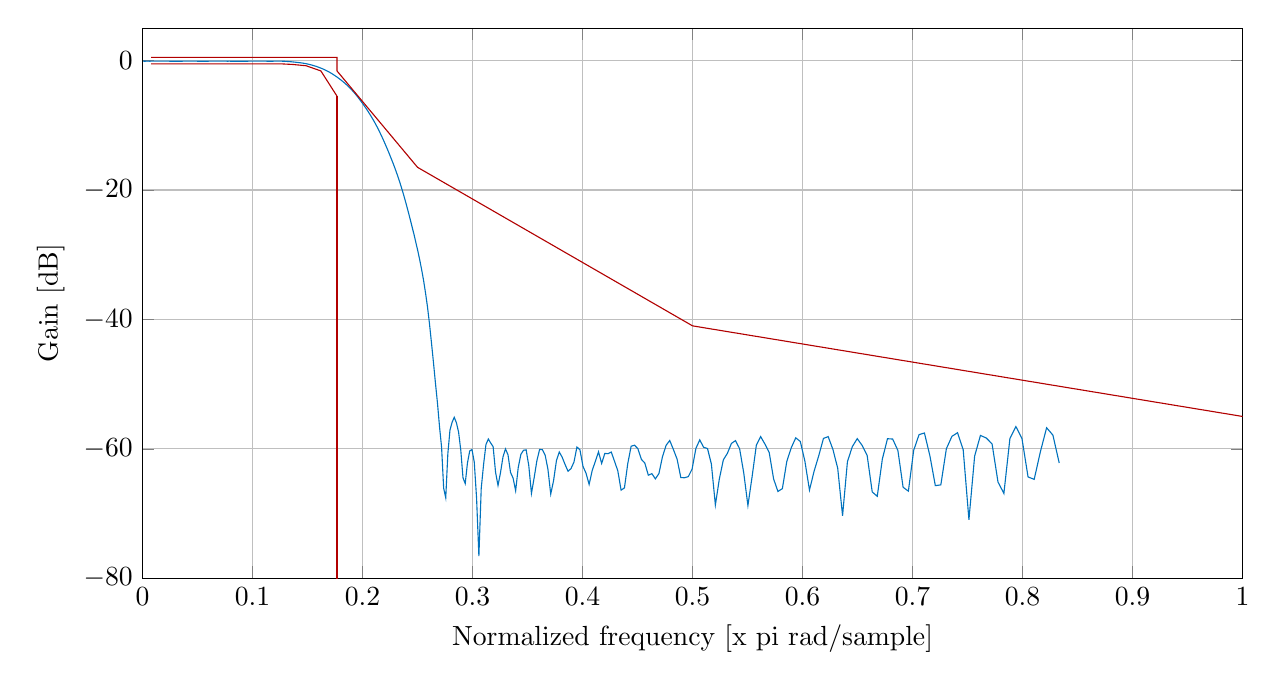
\begin{tikzpicture}

\begin{axis}[%
width=5.5in,
height=2.75in,
at={(0.758in,0.481in)},
scale only axis,
xmin=0,
xmax=1,
xlabel={Normalized frequency [x pi rad/sample]},
xmajorgrids,
ymin=-80,
ymax=5,
ylabel={Gain [dB]},
ymajorgrids,
axis background/.style={fill=white}
]
\addplot [color=mycolor1,solid,forget plot]
  table[row sep=crcr]{%
0.000833333333333333	-0.097036\\
0.000839125	-0.0967\\
0.000844958333333333	-0.097207\\
0.000850791666666667	-0.096769\\
0.000856708333333333	-0.096474\\
0.000862666666666667	-0.095963\\
0.000868625	-0.095232\\
0.000874666666666667	-0.095679\\
0.00088075	-0.095369\\
0.000886833333333333	-0.095159\\
0.000893	-0.095252\\
0.000899208333333333	-0.09498\\
0.000905416666666667	-0.095305\\
0.000911708333333333	-0.095367\\
0.000918041666666667	-0.095283\\
0.000924416666666667	-0.094896\\
0.000930833333333333	-0.094782\\
0.000937291666666667	-0.094842\\
0.000943791666666667	-0.094698\\
0.000950333333333333	-0.094553\\
0.000956916666666667	-0.094738\\
0.000963583333333333	-0.094124\\
0.00097025	-0.094646\\
0.000977	-0.094053\\
0.00098375	-0.094028\\
0.000990583333333333	-0.094229\\
0.000997458333333333	-0.094548\\
0.001004375	-0.09441\\
0.00101133333333333	-0.09426\\
0.001018375	-0.094895\\
0.00102541666666667	-0.094462\\
0.00103254166666667	-0.094314\\
0.00103970833333333	-0.094453\\
0.00104691666666667	-0.094619\\
0.00105420833333333	-0.094429\\
0.0010615	-0.094434\\
0.001068875	-0.094579\\
0.00107629166666667	-0.094338\\
0.00108375	-0.094389\\
0.00109129166666667	-0.094061\\
0.00109883333333333	-0.094594\\
0.00110645833333333	-0.094354\\
0.00111416666666667	-0.09419\\
0.001121875	-0.094164\\
0.00112966666666667	-0.094676\\
0.0011375	-0.094332\\
0.00114541666666667	-0.09402\\
0.00115333333333333	-0.0943\\
0.00116133333333333	-0.094369\\
0.00116941666666667	-0.0945\\
0.00117754166666667	-0.093477\\
0.00118570833333333	-0.094414\\
0.00119391666666667	-0.093867\\
0.00120220833333333	-0.094073\\
0.00121054166666667	-0.094437\\
0.00121895833333333	-0.093863\\
0.00122741666666667	-0.09412\\
0.00123591666666667	-0.093982\\
0.0012445	-0.094171\\
0.001253125	-0.094323\\
0.00126183333333333	-0.094928\\
0.00127058333333333	-0.094738\\
0.00127941666666667	-0.094044\\
0.00128829166666667	-0.094248\\
0.00129720833333333	-0.094441\\
0.00130620833333333	-0.09461\\
0.00131529166666667	-0.093899\\
0.00132441666666667	-0.09453\\
0.00133358333333333	-0.094629\\
0.00134283333333333	-0.094398\\
0.00135216666666667	-0.094021\\
0.00136154166666667	-0.094618\\
0.001371	-0.094115\\
0.0013805	-0.094451\\
0.00139008333333333	-0.093973\\
0.00139970833333333	-0.094361\\
0.00140945833333333	-0.093998\\
0.00141920833333333	-0.094393\\
0.00142908333333333	-0.09378\\
0.001439	-0.094319\\
0.00144895833333333	-0.094036\\
0.00145904166666667	-0.093727\\
0.00146916666666667	-0.094122\\
0.00147933333333333	-0.094292\\
0.001489625	-0.094141\\
0.00149995833333333	-0.094634\\
0.00151033333333333	-0.093805\\
0.00152083333333333	-0.094181\\
0.001531375	-0.094431\\
0.001542	-0.093785\\
0.00155270833333333	-0.094163\\
0.00156345833333333	-0.094276\\
0.00157433333333333	-0.093554\\
0.00158525	-0.093829\\
0.00159625	-0.09409\\
0.00160733333333333	-0.094235\\
0.00161845833333333	-0.094602\\
0.00162970833333333	-0.094128\\
0.001641	-0.093834\\
0.00165241666666667	-0.093785\\
0.001663875	-0.093819\\
0.00167541666666667	-0.093576\\
0.00168704166666667	-0.094679\\
0.00169875	-0.093709\\
0.00171054166666667	-0.09436\\
0.00172241666666667	-0.094638\\
0.00173433333333333	-0.094119\\
0.001746375	-0.093842\\
0.0017585	-0.094757\\
0.00177070833333333	-0.094762\\
0.001783	-0.094376\\
0.001795375	-0.092633\\
0.00180783333333333	-0.094576\\
0.001820375	-0.09369\\
0.001833	-0.094792\\
0.00184570833333333	-0.092481\\
0.0018585	-0.094311\\
0.00187141666666667	-0.095378\\
0.00188441666666667	-0.094285\\
0.00189745833333333	-0.094585\\
0.001910625	-0.095024\\
0.00192391666666667	-0.095503\\
0.00193725	-0.094208\\
0.00195070833333333	-0.092351\\
0.00196420833333333	-0.09394\\
0.00197783333333333	-0.093803\\
0.00199158333333333	-0.093508\\
0.00200541666666667	-0.093127\\
0.00201929166666667	-0.095832\\
0.00203333333333333	-0.093764\\
0.00204741666666667	-0.092444\\
0.002061625	-0.092424\\
0.00207595833333333	-0.092451\\
0.00209033333333333	-0.092971\\
0.00210483333333333	-0.092142\\
0.00211945833333333	-0.09265\\
0.00213416666666667	-0.095004\\
0.00214895833333333	-0.094307\\
0.002163875	-0.092512\\
0.002178875	-0.095702\\
0.002194	-0.092576\\
0.00220925	-0.095129\\
0.00222458333333333	-0.093863\\
0.00224	-0.092468\\
0.00225554166666667	-0.093473\\
0.00227120833333333	-0.09444\\
0.00228695833333333	-0.095046\\
0.00230283333333333	-0.095711\\
0.00231879166666667	-0.095204\\
0.002334875	-0.094309\\
0.00235108333333333	-0.093058\\
0.00236741666666667	-0.093682\\
0.00238383333333333	-0.095231\\
0.002400375	-0.093251\\
0.00241704166666667	-0.094117\\
0.00243379166666667	-0.093262\\
0.00245066666666667	-0.09486\\
0.00246770833333333	-0.092621\\
0.00248479166666667	-0.094166\\
0.00250204166666667	-0.094722\\
0.00251941666666667	-0.094589\\
0.002536875	-0.093828\\
0.0025545	-0.093573\\
0.00257220833333333	-0.092867\\
0.00259008333333333	-0.093682\\
0.00260804166666667	-0.094191\\
0.002626125	-0.095299\\
0.002644375	-0.094859\\
0.00266270833333333	-0.093589\\
0.00268116666666667	-0.09384\\
0.00269979166666667	-0.094557\\
0.0027185	-0.093934\\
0.002737375	-0.0939\\
0.002756375	-0.094451\\
0.0027755	-0.093899\\
0.00279475	-0.094593\\
0.00281416666666667	-0.094439\\
0.00283366666666667	-0.094358\\
0.00285333333333333	-0.093514\\
0.002873125	-0.093536\\
0.00289308333333333	-0.094069\\
0.00291316666666667	-0.094076\\
0.002933375	-0.09352\\
0.00295370833333333	-0.094174\\
0.00297420833333333	-0.093705\\
0.00299483333333333	-0.093913\\
0.003015625	-0.094546\\
0.00303654166666667	-0.093446\\
0.003057625	-0.094372\\
0.00307883333333333	-0.093946\\
0.00310020833333333	-0.09471\\
0.00312170833333333	-0.094077\\
0.003143375	-0.094408\\
0.00316516666666667	-0.093872\\
0.003187125	-0.09442\\
0.00320925	-0.094555\\
0.00323154166666667	-0.09356\\
0.00325395833333333	-0.093583\\
0.00327654166666667	-0.094924\\
0.00329925	-0.094736\\
0.00332216666666667	-0.094669\\
0.00334520833333333	-0.094545\\
0.00336841666666667	-0.094825\\
0.00339179166666667	-0.094268\\
0.00341533333333333	-0.09425\\
0.003439	-0.094416\\
0.003462875	-0.094582\\
0.00348691666666667	-0.095161\\
0.00351108333333333	-0.093905\\
0.00353545833333333	-0.094821\\
0.00356	-0.094388\\
0.00358470833333333	-0.093569\\
0.00360958333333333	-0.09435\\
0.003634625	-0.094042\\
0.00365983333333333	-0.094759\\
0.00368520833333333	-0.094232\\
0.00371079166666667	-0.094476\\
0.00373654166666667	-0.094648\\
0.00376245833333333	-0.094723\\
0.00378858333333333	-0.094486\\
0.003814875	-0.094073\\
0.00384133333333333	-0.094178\\
0.003868	-0.094073\\
0.00389483333333333	-0.09466\\
0.00392183333333333	-0.095252\\
0.00394908333333333	-0.095315\\
0.00397645833333333	-0.095391\\
0.00400404166666667	-0.094806\\
0.00403183333333333	-0.095319\\
0.00405983333333333	-0.094877\\
0.004088	-0.094586\\
0.00411633333333333	-0.09401\\
0.00414491666666667	-0.094908\\
0.00417375	-0.094767\\
0.0042025	-0.094584\\
0.00423166666666667	-0.094835\\
0.00426125	-0.095442\\
0.00429083333333333	-0.095072\\
0.00432041666666667	-0.095121\\
0.00435041666666667	-0.095958\\
0.00438083333333333	-0.09493\\
0.00441125	-0.095309\\
0.00444166666666667	-0.095062\\
0.0044725	-0.095761\\
0.00450333333333333	-0.095544\\
0.00453458333333333	-0.095932\\
0.00456625	-0.095596\\
0.00459791666666667	-0.095273\\
0.00463	-0.095781\\
0.00466208333333333	-0.095443\\
0.00469416666666667	-0.09567\\
0.00472666666666667	-0.095303\\
0.00475958333333333	-0.095172\\
0.0047925	-0.095495\\
0.00482583333333333	-0.094898\\
0.00485958333333333	-0.095519\\
0.00489333333333333	-0.095429\\
0.00492708333333333	-0.096029\\
0.00496125	-0.095393\\
0.00499583333333333	-0.096351\\
0.00503041666666667	-0.096141\\
0.00506541666666667	-0.096077\\
0.00510041666666667	-0.09638\\
0.00513583333333333	-0.095148\\
0.00517125	-0.095773\\
0.0052075	-0.094713\\
0.00524333333333333	-0.095419\\
0.00528	-0.09563\\
0.00531666666666667	-0.095575\\
0.00535333333333333	-0.095444\\
0.00539041666666667	-0.096149\\
0.00542791666666667	-0.095655\\
0.00546541666666667	-0.095573\\
0.00550333333333333	-0.095944\\
0.00554166666666667	-0.095976\\
0.00558	-0.095635\\
0.00561875	-0.095453\\
0.00565791666666667	-0.095775\\
0.00569708333333333	-0.095612\\
0.00573666666666667	-0.095895\\
0.00577625	-0.095382\\
0.00581666666666667	-0.095336\\
0.00585666666666667	-0.095516\\
0.0058975	-0.096256\\
0.00593833333333333	-0.095753\\
0.00597958333333333	-0.095521\\
0.00602125	-0.095914\\
0.00606291666666667	-0.095638\\
0.006105	-0.095738\\
0.0061475	-0.096499\\
0.00619	-0.09631\\
0.00623291666666667	-0.095164\\
0.00627625	-0.096784\\
0.00631958333333333	-0.095307\\
0.00636375	-0.09661\\
0.00640791666666667	-0.095776\\
0.00645208333333333	-0.09566\\
0.00649708333333333	-0.094986\\
0.00654208333333333	-0.096542\\
0.0065875	-0.095827\\
0.00663333333333333	-0.097092\\
0.00667916666666667	-0.096761\\
0.00672541666666667	-0.096636\\
0.00677208333333333	-0.095513\\
0.00681916666666667	-0.095638\\
0.00686666666666667	-0.09646\\
0.00691416666666667	-0.095672\\
0.00696208333333333	-0.095515\\
0.00701041666666667	-0.096082\\
0.00705916666666667	-0.09606\\
0.00710791666666667	-0.095781\\
0.0071575	-0.096882\\
0.00720708333333333	-0.096246\\
0.00725708333333333	-0.096532\\
0.0073075	-0.095446\\
0.00735791666666667	-0.096432\\
0.00740916666666667	-0.095836\\
0.00746041666666667	-0.095116\\
0.0075125	-0.095936\\
0.00756458333333333	-0.095752\\
0.00761708333333333	-0.096119\\
0.00766958333333333	-0.095557\\
0.00772291666666667	-0.09556\\
0.00777666666666667	-0.095997\\
0.00783041666666667	-0.095266\\
0.007885	-0.095394\\
0.00793958333333333	-0.095646\\
0.00799458333333333	-0.095742\\
0.00805	-0.095007\\
0.00810583333333333	-0.09579\\
0.00816208333333333	-0.095132\\
0.00821875	-0.095283\\
0.00827583333333333	-0.094738\\
0.00833333333333333	-0.094661\\
0.00839125	-0.094647\\
0.00844958333333333	-0.09489\\
0.00850791666666667	-0.095796\\
0.00856708333333333	-0.095316\\
0.00862666666666667	-0.096173\\
0.00868625	-0.095652\\
0.00874666666666667	-0.095684\\
0.0088075	-0.095733\\
0.00886833333333333	-0.095743\\
0.00893	-0.096511\\
0.00899208333333333	-0.09548\\
0.00905416666666667	-0.095056\\
0.00911708333333333	-0.094994\\
0.00918041666666667	-0.095586\\
0.00924416666666667	-0.095827\\
0.00930833333333333	-0.095071\\
0.00937291666666667	-0.09474\\
0.00943791666666667	-0.093863\\
0.00950333333333333	-0.094009\\
0.00956916666666667	-0.095311\\
0.00963583333333333	-0.095097\\
0.0097025	-0.094307\\
0.00977	-0.094884\\
0.0098375	-0.093653\\
0.00990583333333333	-0.094507\\
0.00997458333333333	-0.094264\\
0.01004375	-0.094126\\
0.0101133333333333	-0.093537\\
0.01018375	-0.094769\\
0.0102541666666667	-0.092873\\
0.0103254166666667	-0.093939\\
0.0103970833333333	-0.093115\\
0.0104691666666667	-0.093225\\
0.0105420833333333	-0.093318\\
0.010615	-0.093214\\
0.01068875	-0.093139\\
0.0107629166666667	-0.091641\\
0.0108375	-0.091952\\
0.0109129166666667	-0.092876\\
0.0109883333333333	-0.093582\\
0.0110645833333333	-0.092338\\
0.0111416666666667	-0.092895\\
0.01121875	-0.093428\\
0.0112966666666667	-0.092385\\
0.011375	-0.091932\\
0.0114541666666667	-0.092835\\
0.0115333333333333	-0.092083\\
0.0116133333333333	-0.091645\\
0.0116941666666667	-0.091589\\
0.0117754166666667	-0.091976\\
0.0118570833333333	-0.091875\\
0.0119391666666667	-0.091059\\
0.0120220833333333	-0.091391\\
0.0121054166666667	-0.091503\\
0.0121895833333333	-0.09137\\
0.0122741666666667	-0.091328\\
0.0123591666666667	-0.091265\\
0.012445	-0.090905\\
0.01253125	-0.090332\\
0.0126183333333333	-0.090185\\
0.0127058333333333	-0.090275\\
0.0127941666666667	-0.090891\\
0.0128829166666667	-0.090738\\
0.0129720833333333	-0.089549\\
0.0130620833333333	-0.090393\\
0.0131529166666667	-0.090045\\
0.0132441666666667	-0.089575\\
0.0133358333333333	-0.088879\\
0.0134283333333333	-0.090049\\
0.0135216666666667	-0.089092\\
0.0136154166666667	-0.089566\\
0.01371	-0.088853\\
0.013805	-0.089964\\
0.0139008333333333	-0.088425\\
0.0139970833333333	-0.088179\\
0.0140945833333333	-0.088556\\
0.0141920833333333	-0.087071\\
0.0142908333333333	-0.088511\\
0.01439	-0.087326\\
0.0144895833333333	-0.088378\\
0.0145904166666667	-0.088025\\
0.0146916666666667	-0.086627\\
0.0147933333333333	-0.087457\\
0.01489625	-0.087161\\
0.0149995833333333	-0.086273\\
0.0151033333333333	-0.087019\\
0.0152083333333333	-0.086887\\
0.01531375	-0.086753\\
0.01542	-0.08638\\
0.0155270833333333	-0.085915\\
0.0156345833333333	-0.085728\\
0.0157433333333333	-0.085434\\
0.0158525	-0.084944\\
0.0159625	-0.085968\\
0.0160733333333333	-0.085661\\
0.0161845833333333	-0.086\\
0.0162970833333333	-0.084862\\
0.01641	-0.085573\\
0.0165241666666667	-0.085057\\
0.01663875	-0.085377\\
0.0167541666666667	-0.085347\\
0.0168704166666667	-0.084825\\
0.0169875	-0.085113\\
0.0171054166666667	-0.085008\\
0.0172241666666667	-0.085544\\
0.0173433333333333	-0.084945\\
0.01746375	-0.084077\\
0.017585	-0.084831\\
0.0177070833333333	-0.084873\\
0.01783	-0.08532\\
0.01795375	-0.085039\\
0.0180783333333333	-0.08412\\
0.01820375	-0.084939\\
0.01833	-0.084781\\
0.0184570833333333	-0.084167\\
0.018585	-0.08579\\
0.0187141666666667	-0.084592\\
0.0188441666666667	-0.085853\\
0.0189745833333333	-0.0841\\
0.01910625	-0.08439\\
0.0192391666666667	-0.084638\\
0.0193725	-0.085764\\
0.0195070833333333	-0.085618\\
0.0196420833333333	-0.086167\\
0.0197783333333333	-0.085521\\
0.0199158333333333	-0.086157\\
0.0200541666666667	-0.085664\\
0.0201929166666667	-0.085582\\
0.0203333333333333	-0.085361\\
0.0204741666666667	-0.086332\\
0.02061625	-0.087024\\
0.0207595833333333	-0.087167\\
0.0209033333333333	-0.08864\\
0.0210483333333333	-0.086945\\
0.0211945833333333	-0.088214\\
0.0213416666666667	-0.088537\\
0.0214895833333333	-0.089822\\
0.02163875	-0.089243\\
0.02178875	-0.08954\\
0.02194	-0.089993\\
0.0220925	-0.09093\\
0.0222458333333333	-0.090734\\
0.0224	-0.092316\\
0.0225554166666667	-0.09228\\
0.0227120833333333	-0.091514\\
0.0228695833333333	-0.091665\\
0.0230283333333333	-0.092387\\
0.0231879166666667	-0.092877\\
0.02334875	-0.093764\\
0.0235108333333333	-0.094747\\
0.0236741666666667	-0.094613\\
0.0238383333333333	-0.09562\\
0.02400375	-0.095869\\
0.0241704166666667	-0.096602\\
0.0243379166666667	-0.09632\\
0.0245066666666667	-0.097821\\
0.0246770833333333	-0.097733\\
0.0248479166666667	-0.098722\\
0.0250204166666667	-0.099948\\
0.0251941666666667	-0.10013\\
0.02536875	-0.10014\\
0.025545	-0.10108\\
0.0257220833333333	-0.10123\\
0.0259008333333333	-0.10215\\
0.0260804166666667	-0.10338\\
0.02626125	-0.10273\\
0.02644375	-0.1031\\
0.0266270833333333	-0.10478\\
0.0268116666666667	-0.10516\\
0.0269979166666667	-0.10634\\
0.027185	-0.10599\\
0.02737375	-0.10666\\
0.02756375	-0.10634\\
0.027755	-0.10706\\
0.0279475	-0.10671\\
0.0281416666666667	-0.10724\\
0.0283366666666667	-0.10788\\
0.0285333333333333	-0.10919\\
0.02873125	-0.10922\\
0.0289308333333333	-0.10908\\
0.0291316666666667	-0.1093\\
0.02933375	-0.11053\\
0.0295370833333333	-0.11051\\
0.0297420833333333	-0.11038\\
0.0299483333333333	-0.11097\\
0.03015625	-0.11085\\
0.0303654166666667	-0.111\\
0.03057625	-0.11135\\
0.0307883333333333	-0.11018\\
0.0310020833333333	-0.11088\\
0.0312170833333333	-0.10996\\
0.03143375	-0.11025\\
0.0316516666666667	-0.11044\\
0.03187125	-0.10979\\
0.0320925	-0.11016\\
0.0323154166666667	-0.10937\\
0.0325395833333333	-0.10961\\
0.0327654166666667	-0.10784\\
0.0329925	-0.10773\\
0.0332216666666667	-0.10742\\
0.0334520833333333	-0.10727\\
0.0336841666666667	-0.1051\\
0.0339179166666667	-0.10504\\
0.0341533333333333	-0.10486\\
0.03439	-0.10348\\
0.03462875	-0.10283\\
0.0348691666666667	-0.10214\\
0.0351108333333333	-0.10144\\
0.0353545833333333	-0.10022\\
0.0356	-0.099554\\
0.0358470833333333	-0.099037\\
0.0360958333333333	-0.096969\\
0.03634625	-0.097265\\
0.0365983333333333	-0.096076\\
0.0368520833333333	-0.094466\\
0.0371079166666667	-0.093158\\
0.0373654166666667	-0.091693\\
0.0376245833333333	-0.091955\\
0.0378858333333333	-0.090732\\
0.03814875	-0.090842\\
0.0384133333333333	-0.08853\\
0.03868	-0.087704\\
0.0389483333333333	-0.087992\\
0.0392183333333333	-0.08674\\
0.0394908333333333	-0.085176\\
0.0397645833333333	-0.084453\\
0.0400404166666667	-0.083673\\
0.0403183333333333	-0.082842\\
0.0405983333333333	-0.081792\\
0.04088	-0.081476\\
0.0411633333333333	-0.081971\\
0.0414491666666667	-0.08118\\
0.0417375	-0.081087\\
0.042025	-0.081094\\
0.0423166666666667	-0.080761\\
0.0426125	-0.080982\\
0.0429083333333333	-0.080275\\
0.0432041666666667	-0.08041\\
0.0435041666666667	-0.080446\\
0.0438083333333333	-0.081138\\
0.0441125	-0.081462\\
0.0444166666666667	-0.081305\\
0.044725	-0.082094\\
0.0450333333333333	-0.082689\\
0.0453458333333333	-0.083162\\
0.0456625	-0.084122\\
0.0459791666666667	-0.085463\\
0.0463	-0.085628\\
0.0466208333333333	-0.087198\\
0.0469416666666667	-0.087895\\
0.0472666666666667	-0.089578\\
0.0475958333333333	-0.09096\\
0.047925	-0.092208\\
0.0482583333333333	-0.092205\\
0.0485958333333333	-0.093805\\
0.0489333333333333	-0.09399\\
0.0492708333333333	-0.094907\\
0.0496125	-0.096876\\
0.0499583333333333	-0.097953\\
0.0503041666666667	-0.099153\\
0.0506541666666667	-0.10054\\
0.0510041666666667	-0.10055\\
0.0513583333333333	-0.10176\\
0.0517125	-0.1033\\
0.052075	-0.1033\\
0.0524333333333333	-0.10487\\
0.0528	-0.10539\\
0.0531666666666667	-0.10494\\
0.0535333333333333	-0.10433\\
0.0539041666666667	-0.10617\\
0.0542791666666667	-0.10614\\
0.0546541666666667	-0.10574\\
0.0550333333333333	-0.10588\\
0.0554166666666667	-0.10496\\
0.0558	-0.10529\\
0.0561875	-0.10486\\
0.0565791666666667	-0.10382\\
0.0569708333333333	-0.10402\\
0.0573666666666667	-0.10345\\
0.0577625	-0.10187\\
0.0581666666666667	-0.10081\\
0.0585666666666667	-0.10019\\
0.058975	-0.099225\\
0.0593833333333333	-0.098457\\
0.0597958333333333	-0.098117\\
0.0602125	-0.096129\\
0.0606291666666667	-0.094529\\
0.06105	-0.094464\\
0.061475	-0.092934\\
0.0619	-0.092315\\
0.0623291666666667	-0.090136\\
0.0627625	-0.089811\\
0.0631958333333333	-0.089031\\
0.0636375	-0.088328\\
0.0640791666666667	-0.087151\\
0.0645208333333333	-0.087005\\
0.0649708333333333	-0.087268\\
0.0654208333333333	-0.085605\\
0.065875	-0.085477\\
0.0663333333333333	-0.085455\\
0.0667916666666667	-0.086121\\
0.0672541666666667	-0.085887\\
0.0677208333333333	-0.085531\\
0.0681916666666667	-0.086683\\
0.0686666666666667	-0.086514\\
0.0691416666666667	-0.086706\\
0.0696208333333333	-0.088442\\
0.0701041666666667	-0.088312\\
0.0705916666666667	-0.089068\\
0.0710791666666667	-0.089819\\
0.071575	-0.090582\\
0.0720708333333333	-0.091361\\
0.0725708333333333	-0.091958\\
0.073075	-0.09262\\
0.0735791666666667	-0.091927\\
0.0740916666666667	-0.093715\\
0.0746041666666667	-0.094231\\
0.075125	-0.094854\\
0.0756458333333333	-0.095063\\
0.0761708333333333	-0.095649\\
0.0766958333333333	-0.096817\\
0.0772291666666667	-0.097145\\
0.0777666666666667	-0.097443\\
0.0783041666666667	-0.096196\\
0.07885	-0.096521\\
0.0793958333333333	-0.096667\\
0.0799458333333333	-0.097165\\
0.0805	-0.098481\\
0.0810583333333333	-0.097116\\
0.0816208333333333	-0.096877\\
0.0821875	-0.097538\\
0.0827583333333333	-0.097309\\
0.0833333333333333	-0.09845\\
0.0839125	-0.099261\\
0.0844958333333333	-0.098361\\
0.0850791666666667	-0.099834\\
0.0856708333333333	-0.1008\\
0.0862666666666667	-0.10052\\
0.0868625	-0.10149\\
0.0874666666666667	-0.10211\\
0.088075	-0.10216\\
0.0886833333333333	-0.10289\\
0.0893	-0.10305\\
0.0899208333333333	-0.10355\\
0.0905416666666667	-0.10337\\
0.0911708333333333	-0.10304\\
0.0918041666666667	-0.10336\\
0.0924416666666667	-0.10434\\
0.0930833333333333	-0.10141\\
0.0937291666666667	-0.10186\\
0.0943791666666667	-0.1001\\
0.0950333333333333	-0.099423\\
0.0956916666666667	-0.097612\\
0.0963583333333333	-0.095938\\
0.097025	-0.094333\\
0.0977	-0.092776\\
0.098375	-0.090406\\
0.0990583333333333	-0.088152\\
0.0997458333333333	-0.087306\\
0.1004375	-0.084675\\
0.101133333333333	-0.083607\\
0.1018375	-0.081442\\
0.102541666666667	-0.081149\\
0.103254166666667	-0.079866\\
0.103970833333333	-0.079735\\
0.104691666666667	-0.080083\\
0.105420833333333	-0.080016\\
0.10615	-0.080526\\
0.1068875	-0.082059\\
0.107629166666667	-0.083866\\
0.108375	-0.084577\\
0.109129166666667	-0.086679\\
0.109883333333333	-0.088917\\
0.110645833333333	-0.091851\\
0.111416666666667	-0.092748\\
0.1121875	-0.095292\\
0.112966666666667	-0.097245\\
0.11375	-0.098784\\
0.114541666666667	-0.098736\\
0.115333333333333	-0.09931\\
0.116133333333333	-0.099299\\
0.116941666666667	-0.098681\\
0.117754166666667	-0.098293\\
0.118570833333333	-0.097558\\
0.119391666666667	-0.095207\\
0.120220833333333	-0.094447\\
0.121054166666667	-0.092998\\
0.121895833333333	-0.092148\\
0.122741666666667	-0.090744\\
0.123591666666667	-0.090399\\
0.12445	-0.089837\\
0.1253125	-0.092486\\
0.126183333333333	-0.094205\\
0.127058333333333	-0.097674\\
0.127941666666667	-0.10247\\
0.128829166666667	-0.10852\\
0.129720833333333	-0.11655\\
0.130620833333333	-0.12482\\
0.131529166666667	-0.13521\\
0.132441666666667	-0.14717\\
0.133358333333333	-0.15987\\
0.134283333333333	-0.17249\\
0.135216666666667	-0.18712\\
0.136154166666667	-0.20225\\
0.1371	-0.21853\\
0.13805	-0.23435\\
0.139008333333333	-0.2515\\
0.139970833333333	-0.26948\\
0.140945833333333	-0.28804\\
0.141920833333333	-0.30772\\
0.142908333333333	-0.3283\\
0.1439	-0.35144\\
0.144895833333333	-0.37561\\
0.145904166666667	-0.40091\\
0.146916666666667	-0.43001\\
0.147933333333333	-0.45954\\
0.1489625	-0.49283\\
0.149995833333333	-0.53198\\
0.151033333333333	-0.57\\
0.152083333333333	-0.61316\\
0.1531375	-0.65976\\
0.1542	-0.70835\\
0.155270833333333	-0.75996\\
0.156345833333333	-0.81682\\
0.157433333333333	-0.87547\\
0.158525	-0.93731\\
0.159625	-1.0037\\
0.160733333333333	-1.0745\\
0.161845833333333	-1.1476\\
0.162970833333333	-1.2251\\
0.1641	-1.3073\\
0.165241666666667	-1.3944\\
0.1663875	-1.4862\\
0.167541666666667	-1.5842\\
0.168704166666667	-1.687\\
0.169875	-1.7959\\
0.171054166666667	-1.9119\\
0.172241666666667	-2.0343\\
0.173433333333333	-2.1625\\
0.1746375	-2.2963\\
0.17585	-2.437\\
0.177070833333333	-2.5829\\
0.1783	-2.7353\\
0.1795375	-2.8938\\
0.180783333333333	-3.059\\
0.1820375	-3.2298\\
0.1833	-3.4122\\
0.184570833333333	-3.5989\\
0.18585	-3.7973\\
0.187141666666667	-4.004\\
0.188441666666667	-4.2243\\
0.189745833333333	-4.4559\\
0.1910625	-4.6974\\
0.192391666666667	-4.9539\\
0.193725	-5.2224\\
0.195070833333333	-5.5058\\
0.196420833333333	-5.797\\
0.197783333333333	-6.1028\\
0.199158333333333	-6.4183\\
0.200541666666667	-6.7448\\
0.201929166666667	-7.0833\\
0.203333333333333	-7.4309\\
0.204741666666667	-7.7917\\
0.2061625	-8.1681\\
0.207595833333333	-8.5578\\
0.209033333333333	-8.9646\\
0.210483333333333	-9.3943\\
0.211945833333333	-9.8418\\
0.213416666666667	-10.314\\
0.214895833333333	-10.813\\
0.2163875	-11.337\\
0.2178875	-11.88\\
0.2194	-12.447\\
0.220925	-13.039\\
0.222458333333333	-13.645\\
0.224	-14.273\\
0.225554166666667	-14.932\\
0.227120833333333	-15.596\\
0.228695833333333	-16.292\\
0.230283333333333	-17.027\\
0.231879166666667	-17.798\\
0.2334875	-18.619\\
0.235108333333333	-19.477\\
0.236741666666667	-20.399\\
0.238383333333333	-21.372\\
0.2400375	-22.4\\
0.241704166666667	-23.465\\
0.243379166666667	-24.568\\
0.245066666666667	-25.724\\
0.246770833333333	-26.871\\
0.248479166666667	-28.124\\
0.250204166666667	-29.383\\
0.251941666666667	-30.777\\
0.2536875	-32.277\\
0.25545	-33.942\\
0.257220833333333	-35.884\\
0.259008333333333	-38.024\\
0.260804166666667	-40.603\\
0.2626125	-43.537\\
0.2644375	-46.611\\
0.266270833333333	-49.841\\
0.268116666666667	-52.938\\
0.269979166666667	-56.592\\
0.27185	-59.748\\
0.2737375	-66.091\\
0.2756375	-67.572\\
0.27755	-60.745\\
0.279475	-57.108\\
0.281416666666667	-55.9\\
0.283366666666667	-55.129\\
0.285333333333333	-55.97\\
0.2873125	-57.422\\
0.289308333333333	-60.225\\
0.291316666666667	-64.485\\
0.2933375	-65.372\\
0.295370833333333	-62.196\\
0.297420833333333	-60.331\\
0.299483333333333	-60.113\\
0.3015625	-62.062\\
0.303654166666667	-67.592\\
0.3057625	-76.591\\
0.307883333333333	-66.133\\
0.310020833333333	-62.436\\
0.312170833333333	-59.356\\
0.3143375	-58.489\\
0.316516666666667	-59.108\\
0.3187125	-59.674\\
0.320925	-63.637\\
0.323154166666667	-65.667\\
0.325395833333333	-63.706\\
0.327654166666667	-61.265\\
0.329925	-60.016\\
0.332216666666667	-60.917\\
0.334520833333333	-63.648\\
0.336841666666667	-64.52\\
0.339179166666667	-66.476\\
0.341533333333333	-62.889\\
0.3439	-60.877\\
0.3462875	-60.232\\
0.348691666666667	-60.153\\
0.351108333333333	-62.571\\
0.353545833333333	-66.897\\
0.356	-64.476\\
0.358470833333333	-61.847\\
0.360958333333333	-60.103\\
0.3634625	-60.13\\
0.365983333333333	-60.963\\
0.368520833333333	-63.139\\
0.371079166666667	-67.002\\
0.373654166666667	-64.919\\
0.376245833333333	-61.842\\
0.378858333333333	-60.501\\
0.3814875	-61.301\\
0.384133333333333	-62.436\\
0.3868	-63.465\\
0.389483333333333	-63.064\\
0.392183333333333	-62.06\\
0.394908333333333	-59.722\\
0.397645833333333	-60.167\\
0.400404166666667	-62.72\\
0.403183333333333	-63.785\\
0.405983333333333	-65.508\\
0.4088	-63.334\\
0.411633333333333	-61.94\\
0.414491666666667	-60.46\\
0.417375	-62.265\\
0.42025	-60.71\\
0.423166666666667	-60.758\\
0.426125	-60.506\\
0.429083333333333	-61.937\\
0.432041666666667	-63.392\\
0.435041666666667	-66.392\\
0.438083333333333	-66.045\\
0.441125	-62.265\\
0.444166666666667	-59.601\\
0.44725	-59.445\\
0.450333333333333	-59.989\\
0.453458333333333	-61.626\\
0.456625	-62.21\\
0.459791666666667	-64.083\\
0.463	-63.84\\
0.466208333333333	-64.642\\
0.469416666666667	-63.836\\
0.472666666666667	-61.218\\
0.475958333333333	-59.467\\
0.47925	-58.715\\
0.482583333333333	-60.1\\
0.485958333333333	-61.6\\
0.489333333333333	-64.453\\
0.492708333333333	-64.471\\
0.496125	-64.305\\
0.499583333333333	-63.133\\
0.503041666666667	-59.937\\
0.506541666666667	-58.628\\
0.510041666666667	-59.754\\
0.513583333333333	-59.954\\
0.517125	-62.359\\
0.52075	-68.685\\
0.524333333333333	-64.684\\
0.528	-61.705\\
0.531666666666667	-60.703\\
0.535333333333333	-59.169\\
0.539041666666667	-58.734\\
0.542791666666667	-59.989\\
0.546541666666667	-63.73\\
0.550333333333333	-68.768\\
0.554166666666667	-64.276\\
0.558	-59.433\\
0.561875	-58.106\\
0.565791666666667	-59.267\\
0.569708333333333	-60.587\\
0.573666666666667	-64.649\\
0.577625	-66.597\\
0.581666666666667	-66.15\\
0.585666666666667	-61.955\\
0.58975	-59.826\\
0.593833333333333	-58.304\\
0.597958333333333	-58.865\\
0.602125	-61.909\\
0.606291666666667	-66.38\\
0.6105	-63.462\\
0.61475	-61.052\\
0.619	-58.398\\
0.623291666666667	-58.116\\
0.627625	-60.104\\
0.631958333333333	-63.006\\
0.636375	-70.341\\
0.640791666666667	-62.001\\
0.645208333333333	-59.676\\
0.649708333333333	-58.428\\
0.654208333333333	-59.484\\
0.65875	-61.048\\
0.663333333333333	-66.663\\
0.667916666666667	-67.341\\
0.672541666666667	-61.585\\
0.677208333333333	-58.442\\
0.681916666666667	-58.492\\
0.686666666666667	-60.25\\
0.691416666666667	-65.946\\
0.696208333333333	-66.543\\
0.701041666666667	-60.233\\
0.705916666666667	-57.809\\
0.710791666666667	-57.553\\
0.71575	-61.064\\
0.720708333333333	-65.693\\
0.725708333333333	-65.575\\
0.73075	-59.982\\
0.735791666666667	-58.076\\
0.740916666666667	-57.511\\
0.746041666666667	-60.144\\
0.75125	-70.958\\
0.756458333333333	-61.113\\
0.761708333333333	-57.936\\
0.766958333333333	-58.325\\
0.772291666666667	-59.24\\
0.777666666666667	-65.131\\
0.783041666666667	-66.892\\
0.7885	-58.422\\
0.793958333333333	-56.564\\
0.799458333333333	-58.404\\
0.805	-64.348\\
0.810583333333333	-64.723\\
0.816208333333333	-60.454\\
0.821875	-56.747\\
0.827583333333333	-57.879\\
0.833333333333333	-62.194\\
};
\addplot [color=black!30!red,solid,forget plot]
  table[row sep=crcr]{%
0.1768	-5.5\\
0.1768	-88.5\\
};
\addplot [color=black!30!red,solid,forget plot]
  table[row sep=crcr]{%
0.0078125	0.5\\
0.015625	0.5\\
0.03125	0.5\\
0.0625	0.5\\
0.0883883476483184	0.5\\
0.0963881765879963	0.5\\
0.105112051906714	0.5\\
0.114625505400584	0.5\\
0.125	0.5\\
0.136313466583157	0.5\\
0.14865088937534	0.5\\
0.162104944331376	0.5\\
0.176776695296637	0.5\\
0.176776695296637	-1.6\\
0.25	-16.5\\
0.5	-41\\
1	-55\\
1.1	-55.5\\
};
\addplot [color=black!30!red,solid,forget plot]
  table[row sep=crcr]{%
0.0078125	-0.5\\
0.015625	-0.5\\
0.03125	-0.5\\
0.0625	-0.5\\
0.0883883476483184	-0.5\\
0.0963881765879963	-0.5\\
0.105112051906714	-0.5\\
0.114625505400584	-0.5\\
0.125	-0.5\\
0.136313466583157	-0.6\\
0.14865088937534	-0.8\\
0.162104944331376	-1.6\\
0.176776695296637	-5.5\\
0.176776695296637	-5.5\\
};
\end{axis}
\end{tikzpicture}%
	\caption{Decimation magnitude response with requirements.}
	\label{fig:acceptDecMag}
\end{figure}
\begin{figure}[H]
	\centering
	\tikzsetnextfilename{acceptDecPhase}
	% This file was created by matlab2tikz.
%
%The latest updates can be retrieved from
%  http://www.mathworks.com/matlabcentral/fileexchange/22022-matlab2tikz-matlab2tikz
%where you can also make suggestions and rate matlab2tikz.
%
\definecolor{mycolor1}{rgb}{0.00000,0.44700,0.74100}%
%
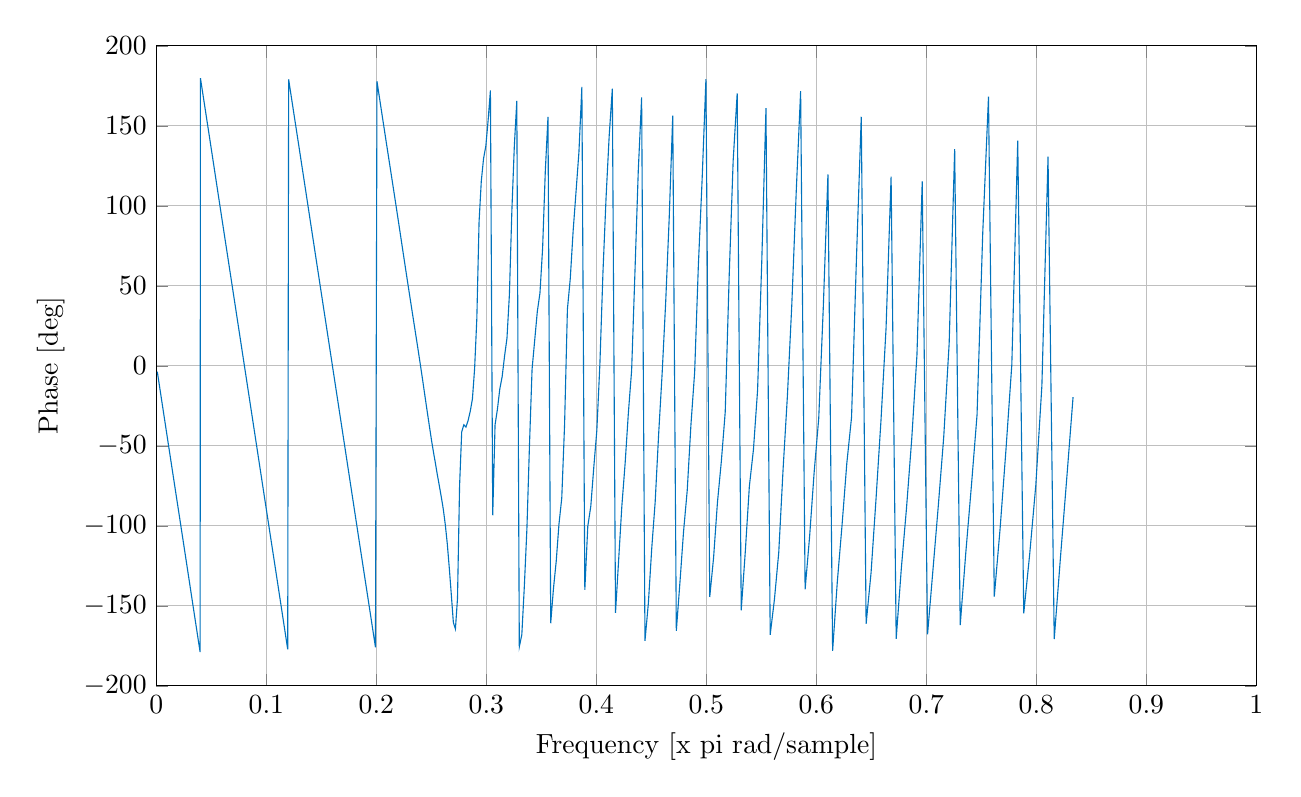
\begin{tikzpicture}

\begin{axis}[%
width=5.5in,
height=3.2in,
at={(0.758in,0.481in)},
scale only axis,
xmin=0,
xmax=1,
xlabel={Frequency [x pi rad/sample]},
xmajorgrids,
ymin=-200,
ymax=200,
ylabel={Phase [deg]},
ymajorgrids,
axis background/.style={fill=white}
]
\addplot [color=mycolor1,solid,forget plot]
  table[row sep=crcr]{%
0.000833333333333333	-3.6514\\
0.000839125	-3.6779\\
0.000844958333333333	-3.7048\\
0.000850791666666667	-3.7318\\
0.000856708333333333	-3.7583\\
0.000862666666666667	-3.7869\\
0.000868625	-3.8167\\
0.000874666666666667	-3.8421\\
0.00088075	-3.8685\\
0.000886833333333333	-3.9024\\
0.000893	-3.9259\\
0.000899208333333333	-3.9516\\
0.000905416666666667	-3.9856\\
0.000911708333333333	-4.0135\\
0.000918041666666667	-4.0424\\
0.000924416666666667	-4.0753\\
0.000930833333333333	-4.1029\\
0.000937291666666667	-4.1304\\
0.000943791666666667	-4.16\\
0.000950333333333333	-4.1905\\
0.000956916666666667	-4.2205\\
0.000963583333333333	-4.2537\\
0.00097025	-4.2846\\
0.000977	-4.3136\\
0.00098375	-4.3444\\
0.000990583333333333	-4.3778\\
0.000997458333333333	-4.4078\\
0.001004375	-4.4377\\
0.00101133333333333	-4.4669\\
0.001018375	-4.5053\\
0.00102541666666667	-4.5346\\
0.00103254166666667	-4.5693\\
0.00103970833333333	-4.6019\\
0.00104691666666667	-4.6328\\
0.00105420833333333	-4.6672\\
0.0010615	-4.6989\\
0.001068875	-4.7301\\
0.00107629166666667	-4.7666\\
0.00108375	-4.8032\\
0.00109129166666667	-4.8344\\
0.00109883333333333	-4.868\\
0.00110645833333333	-4.9065\\
0.00111416666666667	-4.942\\
0.001121875	-4.9751\\
0.00112966666666667	-5.0104\\
0.0011375	-5.0464\\
0.00114541666666667	-5.0839\\
0.00115333333333333	-5.1193\\
0.00116133333333333	-5.1556\\
0.00116941666666667	-5.1899\\
0.00117754166666667	-5.228\\
0.00118570833333333	-5.2609\\
0.00119391666666667	-5.3024\\
0.00120220833333333	-5.3439\\
0.00121054166666667	-5.3785\\
0.00121895833333333	-5.4209\\
0.00122741666666667	-5.4512\\
0.00123591666666667	-5.4933\\
0.0012445	-5.5331\\
0.001253125	-5.5743\\
0.00126183333333333	-5.6139\\
0.00127058333333333	-5.6501\\
0.00127941666666667	-5.6901\\
0.00128829166666667	-5.7332\\
0.00129720833333333	-5.7745\\
0.00130620833333333	-5.8146\\
0.00131529166666667	-5.855\\
0.00132441666666667	-5.8938\\
0.00133358333333333	-5.9377\\
0.00134283333333333	-5.9815\\
0.00135216666666667	-6.0237\\
0.00136154166666667	-6.0649\\
0.001371	-6.1058\\
0.0013805	-6.1502\\
0.00139008333333333	-6.1979\\
0.00139970833333333	-6.2388\\
0.00140945833333333	-6.2826\\
0.00141920833333333	-6.3262\\
0.00142908333333333	-6.3691\\
0.001439	-6.4172\\
0.00144895833333333	-6.4627\\
0.00145904166666667	-6.511\\
0.00146916666666667	-6.5518\\
0.00147933333333333	-6.5992\\
0.001489625	-6.6451\\
0.00149995833333333	-6.6923\\
0.00151033333333333	-6.7419\\
0.00152083333333333	-6.7888\\
0.001531375	-6.8362\\
0.001542	-6.8868\\
0.00155270833333333	-6.9356\\
0.00156345833333333	-6.9827\\
0.00157433333333333	-7.0309\\
0.00158525	-7.0757\\
0.00159625	-7.1258\\
0.00160733333333333	-7.1775\\
0.00161845833333333	-7.2302\\
0.00162970833333333	-7.2787\\
0.001641	-7.3296\\
0.00165241666666667	-7.3828\\
0.001663875	-7.4366\\
0.00167541666666667	-7.4856\\
0.00168704166666667	-7.543\\
0.00169875	-7.5903\\
0.00171054166666667	-7.6478\\
0.00172241666666667	-7.7049\\
0.00173433333333333	-7.7586\\
0.001746375	-7.8176\\
0.0017585	-7.8726\\
0.00177070833333333	-7.9207\\
0.001783	-7.9703\\
0.001795375	-8.0283\\
0.00180783333333333	-8.0951\\
0.001820375	-8.1395\\
0.001833	-8.2052\\
0.00184570833333333	-8.2565\\
0.0018585	-8.3081\\
0.00187141666666667	-8.3753\\
0.00188441666666667	-8.4373\\
0.00189745833333333	-8.5007\\
0.001910625	-8.5547\\
0.00192391666666667	-8.6107\\
0.00193725	-8.6659\\
0.00195070833333333	-8.7315\\
0.00196420833333333	-8.8055\\
0.00197783333333333	-8.8504\\
0.00199158333333333	-8.9254\\
0.00200541666666667	-8.9725\\
0.00201929166666667	-9.0474\\
0.00203333333333333	-9.1171\\
0.00204741666666667	-9.1736\\
0.002061625	-9.2302\\
0.00207595833333333	-9.2894\\
0.00209033333333333	-9.3525\\
0.00210483333333333	-9.4273\\
0.00211945833333333	-9.4977\\
0.00213416666666667	-9.5684\\
0.00214895833333333	-9.621\\
0.002163875	-9.6993\\
0.002178875	-9.7629\\
0.002194	-9.8318\\
0.00220925	-9.893\\
0.00222458333333333	-9.9798\\
0.00224	-10.039\\
0.00225554166666667	-10.1\\
0.00227120833333333	-10.173\\
0.00228695833333333	-10.249\\
0.00230283333333333	-10.32\\
0.00231879166666667	-10.391\\
0.002334875	-10.458\\
0.00235108333333333	-10.537\\
0.00236741666666667	-10.624\\
0.00238383333333333	-10.692\\
0.002400375	-10.76\\
0.00241704166666667	-10.847\\
0.00243379166666667	-10.912\\
0.00245066666666667	-10.997\\
0.00246770833333333	-11.072\\
0.00248479166666667	-11.14\\
0.00250204166666667	-11.223\\
0.00251941666666667	-11.309\\
0.002536875	-11.381\\
0.0025545	-11.46\\
0.00257220833333333	-11.543\\
0.00259008333333333	-11.626\\
0.00260804166666667	-11.707\\
0.002626125	-11.787\\
0.002644375	-11.862\\
0.00266270833333333	-11.944\\
0.00268116666666667	-12.037\\
0.00269979166666667	-12.112\\
0.0027185	-12.201\\
0.002737375	-12.279\\
0.002756375	-12.375\\
0.0027755	-12.457\\
0.00279475	-12.544\\
0.00281416666666667	-12.634\\
0.00283366666666667	-12.726\\
0.00285333333333333	-12.808\\
0.002873125	-12.896\\
0.00289308333333333	-12.987\\
0.00291316666666667	-13.079\\
0.002933375	-13.169\\
0.00295370833333333	-13.258\\
0.00297420833333333	-13.354\\
0.00299483333333333	-13.45\\
0.003015625	-13.538\\
0.00303654166666667	-13.632\\
0.003057625	-13.728\\
0.00307883333333333	-13.825\\
0.00310020833333333	-13.922\\
0.00312170833333333	-14.017\\
0.003143375	-14.116\\
0.00316516666666667	-14.217\\
0.003187125	-14.311\\
0.00320925	-14.41\\
0.00323154166666667	-14.515\\
0.00325395833333333	-14.616\\
0.00327654166666667	-14.721\\
0.00329925	-14.818\\
0.00332216666666667	-14.926\\
0.00334520833333333	-15.023\\
0.00336841666666667	-15.13\\
0.00339179166666667	-15.234\\
0.00341533333333333	-15.341\\
0.003439	-15.448\\
0.003462875	-15.556\\
0.00348691666666667	-15.664\\
0.00351108333333333	-15.774\\
0.00353545833333333	-15.886\\
0.00356	-15.993\\
0.00358470833333333	-16.107\\
0.00360958333333333	-16.216\\
0.003634625	-16.33\\
0.00365983333333333	-16.442\\
0.00368520833333333	-16.557\\
0.00371079166666667	-16.671\\
0.00373654166666667	-16.787\\
0.00376245833333333	-16.907\\
0.00378858333333333	-17.025\\
0.003814875	-17.146\\
0.00384133333333333	-17.262\\
0.003868	-17.388\\
0.00389483333333333	-17.506\\
0.00392183333333333	-17.622\\
0.00394908333333333	-17.75\\
0.00397645833333333	-17.872\\
0.00400404166666667	-17.997\\
0.00403183333333333	-18.118\\
0.00405983333333333	-18.251\\
0.004088	-18.375\\
0.00411633333333333	-18.498\\
0.00414491666666667	-18.632\\
0.00417375	-18.756\\
0.0042025	-18.888\\
0.00423166666666667	-19.023\\
0.00426125	-19.156\\
0.00429083333333333	-19.288\\
0.00432041666666667	-19.425\\
0.00435041666666667	-19.563\\
0.00438083333333333	-19.691\\
0.00441125	-19.835\\
0.00444166666666667	-19.971\\
0.0044725	-20.112\\
0.00450333333333333	-20.246\\
0.00453458333333333	-20.391\\
0.00456625	-20.54\\
0.00459791666666667	-20.674\\
0.00463	-20.826\\
0.00466208333333333	-20.965\\
0.00469416666666667	-21.103\\
0.00472666666666667	-21.249\\
0.00475958333333333	-21.403\\
0.0047925	-21.55\\
0.00482583333333333	-21.712\\
0.00485958333333333	-21.856\\
0.00489333333333333	-22.002\\
0.00492708333333333	-22.16\\
0.00496125	-22.314\\
0.00499583333333333	-22.469\\
0.00503041666666667	-22.621\\
0.00506541666666667	-22.778\\
0.00510041666666667	-22.941\\
0.00513583333333333	-23.099\\
0.00517125	-23.256\\
0.0052075	-23.42\\
0.00524333333333333	-23.58\\
0.00528	-23.746\\
0.00531666666666667	-23.915\\
0.00535333333333333	-24.077\\
0.00539041666666667	-24.248\\
0.00542791666666667	-24.412\\
0.00546541666666667	-24.587\\
0.00550333333333333	-24.759\\
0.00554166666666667	-24.93\\
0.00558	-25.102\\
0.00561875	-25.276\\
0.00565791666666667	-25.447\\
0.00569708333333333	-25.626\\
0.00573666666666667	-25.813\\
0.00577625	-25.991\\
0.00581666666666667	-26.173\\
0.00585666666666667	-26.351\\
0.0058975	-26.532\\
0.00593833333333333	-26.713\\
0.00597958333333333	-26.901\\
0.00602125	-27.091\\
0.00606291666666667	-27.276\\
0.006105	-27.475\\
0.0061475	-27.659\\
0.00619	-27.849\\
0.00623291666666667	-28.046\\
0.00627625	-28.24\\
0.00631958333333333	-28.438\\
0.00636375	-28.63\\
0.00640791666666667	-28.828\\
0.00645208333333333	-29.032\\
0.00649708333333333	-29.23\\
0.00654208333333333	-29.438\\
0.0065875	-29.647\\
0.00663333333333333	-29.845\\
0.00667916666666667	-30.055\\
0.00672541666666667	-30.269\\
0.00677208333333333	-30.473\\
0.00681916666666667	-30.689\\
0.00686666666666667	-30.9\\
0.00691416666666667	-31.115\\
0.00696208333333333	-31.331\\
0.00701041666666667	-31.551\\
0.00705916666666667	-31.771\\
0.00710791666666667	-31.991\\
0.0071575	-32.214\\
0.00720708333333333	-32.437\\
0.00725708333333333	-32.663\\
0.0073075	-32.889\\
0.00735791666666667	-33.116\\
0.00740916666666667	-33.345\\
0.00746041666666667	-33.576\\
0.0075125	-33.808\\
0.00756458333333333	-34.049\\
0.00761708333333333	-34.282\\
0.00766958333333333	-34.518\\
0.00772291666666667	-34.758\\
0.00777666666666667	-35.007\\
0.00783041666666667	-35.24\\
0.007885	-35.49\\
0.00793958333333333	-35.74\\
0.00799458333333333	-35.984\\
0.00805	-36.235\\
0.00810583333333333	-36.489\\
0.00816208333333333	-36.739\\
0.00821875	-36.997\\
0.00827583333333333	-37.249\\
0.00833333333333333	-37.511\\
0.00839125	-37.769\\
0.00844958333333333	-38.032\\
0.00850791666666667	-38.297\\
0.00856708333333333	-38.56\\
0.00862666666666667	-38.834\\
0.00868625	-39.104\\
0.00874666666666667	-39.378\\
0.0088075	-39.653\\
0.00886833333333333	-39.918\\
0.00893	-40.206\\
0.00899208333333333	-40.482\\
0.00905416666666667	-40.762\\
0.00911708333333333	-41.045\\
0.00918041666666667	-41.336\\
0.00924416666666667	-41.612\\
0.00930833333333333	-41.903\\
0.00937291666666667	-42.197\\
0.00943791666666667	-42.492\\
0.00950333333333333	-42.781\\
0.00956916666666667	-43.077\\
0.00963583333333333	-43.375\\
0.0097025	-43.682\\
0.00977	-43.988\\
0.0098375	-44.29\\
0.00990583333333333	-44.593\\
0.00997458333333333	-44.9\\
0.01004375	-45.213\\
0.0101133333333333	-45.538\\
0.01018375	-45.848\\
0.0102541666666667	-46.172\\
0.0103254166666667	-46.484\\
0.0103970833333333	-46.813\\
0.0104691666666667	-47.132\\
0.0105420833333333	-47.465\\
0.010615	-47.794\\
0.01068875	-48.126\\
0.0107629166666667	-48.46\\
0.0108375	-48.794\\
0.0109129166666667	-49.139\\
0.0109883333333333	-49.476\\
0.0110645833333333	-49.82\\
0.0111416666666667	-50.156\\
0.01121875	-50.504\\
0.0112966666666667	-50.861\\
0.011375	-51.214\\
0.0114541666666667	-51.567\\
0.0115333333333333	-51.929\\
0.0116133333333333	-52.287\\
0.0116941666666667	-52.652\\
0.0117754166666667	-53.019\\
0.0118570833333333	-53.383\\
0.0119391666666667	-53.751\\
0.0120220833333333	-54.129\\
0.0121054166666667	-54.504\\
0.0121895833333333	-54.879\\
0.0122741666666667	-55.26\\
0.0123591666666667	-55.644\\
0.012445	-56.029\\
0.01253125	-56.42\\
0.0126183333333333	-56.809\\
0.0127058333333333	-57.201\\
0.0127941666666667	-57.6\\
0.0128829166666667	-58\\
0.0129720833333333	-58.397\\
0.0130620833333333	-58.807\\
0.0131529166666667	-59.216\\
0.0132441666666667	-59.626\\
0.0133358333333333	-60.044\\
0.0134283333333333	-60.454\\
0.0135216666666667	-60.87\\
0.0136154166666667	-61.298\\
0.01371	-61.721\\
0.013805	-62.143\\
0.0139008333333333	-62.571\\
0.0139970833333333	-63.01\\
0.0140945833333333	-63.447\\
0.0141920833333333	-63.887\\
0.0142908333333333	-64.329\\
0.01439	-64.766\\
0.0144895833333333	-65.215\\
0.0145904166666667	-65.67\\
0.0146916666666667	-66.125\\
0.0147933333333333	-66.594\\
0.01489625	-67.048\\
0.0149995833333333	-67.513\\
0.0151033333333333	-67.984\\
0.0152083333333333	-68.442\\
0.01531375	-68.919\\
0.01542	-69.397\\
0.0155270833333333	-69.871\\
0.0156345833333333	-70.365\\
0.0157433333333333	-70.849\\
0.0158525	-71.344\\
0.0159625	-71.829\\
0.0160733333333333	-72.326\\
0.0161845833333333	-72.827\\
0.0162970833333333	-73.335\\
0.01641	-73.845\\
0.0165241666666667	-74.358\\
0.01663875	-74.868\\
0.0167541666666667	-75.388\\
0.0168704166666667	-75.906\\
0.0169875	-76.439\\
0.0171054166666667	-76.969\\
0.0172241666666667	-77.494\\
0.0173433333333333	-78.033\\
0.01746375	-78.576\\
0.017585	-79.118\\
0.0177070833333333	-79.656\\
0.01783	-80.207\\
0.01795375	-80.763\\
0.0180783333333333	-81.32\\
0.01820375	-81.886\\
0.01833	-82.44\\
0.0184570833333333	-83.021\\
0.018585	-83.593\\
0.0187141666666667	-84.178\\
0.0188441666666667	-84.754\\
0.0189745833333333	-85.345\\
0.01910625	-85.926\\
0.0192391666666667	-86.517\\
0.0193725	-87.123\\
0.0195070833333333	-87.73\\
0.0196420833333333	-88.333\\
0.0197783333333333	-88.942\\
0.0199158333333333	-89.563\\
0.0200541666666667	-90.175\\
0.0201929166666667	-90.803\\
0.0203333333333333	-91.433\\
0.0204741666666667	-92.067\\
0.02061625	-92.698\\
0.0207595833333333	-93.344\\
0.0209033333333333	-93.988\\
0.0210483333333333	-94.639\\
0.0211945833333333	-95.289\\
0.0213416666666667	-95.954\\
0.0214895833333333	-96.614\\
0.02163875	-97.283\\
0.02178875	-97.957\\
0.02194	-98.644\\
0.0220925	-99.324\\
0.0222458333333333	-100.01\\
0.0224	-100.71\\
0.0225554166666667	-101.4\\
0.0227120833333333	-102.1\\
0.0228695833333333	-102.81\\
0.0230283333333333	-103.52\\
0.0231879166666667	-104.24\\
0.02334875	-104.96\\
0.0235108333333333	-105.7\\
0.0236741666666667	-106.42\\
0.0238383333333333	-107.17\\
0.02400375	-107.91\\
0.0241704166666667	-108.66\\
0.0243379166666667	-109.41\\
0.0245066666666667	-110.17\\
0.0246770833333333	-110.94\\
0.0248479166666667	-111.71\\
0.0250204166666667	-112.48\\
0.0251941666666667	-113.27\\
0.02536875	-114.05\\
0.025545	-114.85\\
0.0257220833333333	-115.64\\
0.0259008333333333	-116.45\\
0.0260804166666667	-117.26\\
0.02626125	-118.08\\
0.02644375	-118.89\\
0.0266270833333333	-119.73\\
0.0268116666666667	-120.56\\
0.0269979166666667	-121.39\\
0.027185	-122.24\\
0.02737375	-123.1\\
0.02756375	-123.95\\
0.027755	-124.82\\
0.0279475	-125.69\\
0.0281416666666667	-126.55\\
0.0283366666666667	-127.44\\
0.0285333333333333	-128.33\\
0.02873125	-129.22\\
0.0289308333333333	-130.13\\
0.0291316666666667	-131.03\\
0.02933375	-131.95\\
0.0295370833333333	-132.86\\
0.0297420833333333	-133.8\\
0.0299483333333333	-134.72\\
0.03015625	-135.66\\
0.0303654166666667	-136.61\\
0.03057625	-137.57\\
0.0307883333333333	-138.52\\
0.0310020833333333	-139.49\\
0.0312170833333333	-140.46\\
0.03143375	-141.45\\
0.0316516666666667	-142.43\\
0.03187125	-143.43\\
0.0320925	-144.42\\
0.0323154166666667	-145.43\\
0.0325395833333333	-146.44\\
0.0327654166666667	-147.47\\
0.0329925	-148.5\\
0.0332216666666667	-149.53\\
0.0334520833333333	-150.57\\
0.0336841666666667	-151.62\\
0.0339179166666667	-152.67\\
0.0341533333333333	-153.73\\
0.03439	-154.81\\
0.03462875	-155.88\\
0.0348691666666667	-156.97\\
0.0351108333333333	-158.05\\
0.0353545833333333	-159.15\\
0.0356	-160.26\\
0.0358470833333333	-161.37\\
0.0360958333333333	-162.49\\
0.03634625	-163.61\\
0.0365983333333333	-164.74\\
0.0368520833333333	-165.89\\
0.0371079166666667	-167.04\\
0.0373654166666667	-168.2\\
0.0376245833333333	-169.36\\
0.0378858333333333	-170.54\\
0.03814875	-171.71\\
0.0384133333333333	-172.9\\
0.03868	-174.1\\
0.0389483333333333	-175.3\\
0.0392183333333333	-176.51\\
0.0394908333333333	-177.74\\
0.0397645833333333	-178.95\\
0.0400404166666667	179.8\\
0.0403183333333333	178.56\\
0.0405983333333333	177.3\\
0.04088	176.05\\
0.0411633333333333	174.78\\
0.0414491666666667	173.5\\
0.0417375	172.21\\
0.042025	170.91\\
0.0423166666666667	169.61\\
0.0426125	168.3\\
0.0429083333333333	166.97\\
0.0432041666666667	165.64\\
0.0435041666666667	164.3\\
0.0438083333333333	162.95\\
0.0441125	161.59\\
0.0444166666666667	160.21\\
0.044725	158.85\\
0.0450333333333333	157.45\\
0.0453458333333333	156.06\\
0.0456625	154.64\\
0.0459791666666667	153.22\\
0.0463	151.79\\
0.0466208333333333	150.35\\
0.0469416666666667	148.89\\
0.0472666666666667	147.44\\
0.0475958333333333	145.96\\
0.047925	144.48\\
0.0482583333333333	142.99\\
0.0485958333333333	141.47\\
0.0489333333333333	139.96\\
0.0492708333333333	138.43\\
0.0496125	136.89\\
0.0499583333333333	135.34\\
0.0503041666666667	133.78\\
0.0506541666666667	132.2\\
0.0510041666666667	130.62\\
0.0513583333333333	129.02\\
0.0517125	127.41\\
0.052075	125.79\\
0.0524333333333333	124.16\\
0.0528	122.52\\
0.0531666666666667	120.87\\
0.0535333333333333	119.19\\
0.0539041666666667	117.51\\
0.0542791666666667	115.83\\
0.0546541666666667	114.12\\
0.0550333333333333	112.41\\
0.0554166666666667	110.68\\
0.0558	108.94\\
0.0561875	107.2\\
0.0565791666666667	105.43\\
0.0569708333333333	103.66\\
0.0573666666666667	101.88\\
0.0577625	100.09\\
0.0581666666666667	98.272\\
0.0585666666666667	96.448\\
0.058975	94.618\\
0.0593833333333333	92.771\\
0.0597958333333333	90.917\\
0.0602125	89.045\\
0.0606291666666667	87.17\\
0.06105	85.277\\
0.061475	83.369\\
0.0619	81.449\\
0.0623291666666667	79.527\\
0.0627625	77.585\\
0.0631958333333333	75.63\\
0.0636375	73.658\\
0.0640791666666667	71.678\\
0.0645208333333333	69.683\\
0.0649708333333333	67.671\\
0.0654208333333333	65.646\\
0.065875	63.615\\
0.0663333333333333	61.56\\
0.0667916666666667	59.5\\
0.0672541666666667	57.418\\
0.0677208333333333	55.328\\
0.0681916666666667	53.217\\
0.0686666666666667	51.098\\
0.0691416666666667	48.953\\
0.0696208333333333	46.798\\
0.0701041666666667	44.624\\
0.0705916666666667	42.442\\
0.0710791666666667	40.243\\
0.071575	38.024\\
0.0720708333333333	35.79\\
0.0725708333333333	33.54\\
0.073075	31.276\\
0.0735791666666667	28.999\\
0.0740916666666667	26.697\\
0.0746041666666667	24.389\\
0.075125	22.054\\
0.0756458333333333	19.708\\
0.0761708333333333	17.348\\
0.0766958333333333	14.964\\
0.0772291666666667	12.565\\
0.0777666666666667	10.158\\
0.0783041666666667	7.7281\\
0.07885	5.2838\\
0.0793958333333333	2.8188\\
0.0799458333333333	0.33677\\
0.0805	-2.1548\\
0.0810583333333333	-4.6659\\
0.0816208333333333	-7.1962\\
0.0821875	-9.7477\\
0.0827583333333333	-12.307\\
0.0833333333333333	-14.892\\
0.0839125	-17.494\\
0.0844958333333333	-20.113\\
0.0850791666666667	-22.753\\
0.0856708333333333	-25.403\\
0.0862666666666667	-28.081\\
0.0868625	-30.769\\
0.0874666666666667	-33.488\\
0.088075	-36.222\\
0.0886833333333333	-38.975\\
0.0893	-41.742\\
0.0899208333333333	-44.537\\
0.0905416666666667	-47.355\\
0.0911708333333333	-50.181\\
0.0918041666666667	-53.031\\
0.0924416666666667	-55.908\\
0.0930833333333333	-58.804\\
0.0937291666666667	-61.716\\
0.0943791666666667	-64.646\\
0.0950333333333333	-67.597\\
0.0956916666666667	-70.565\\
0.0963583333333333	-73.56\\
0.097025	-76.566\\
0.0977	-79.598\\
0.098375	-82.651\\
0.0990583333333333	-85.711\\
0.0997458333333333	-88.798\\
0.1004375	-91.901\\
0.101133333333333	-95.026\\
0.1018375	-98.17\\
0.102541666666667	-101.33\\
0.103254166666667	-104.53\\
0.103970833333333	-107.74\\
0.104691666666667	-110.96\\
0.105420833333333	-114.21\\
0.10615	-117.5\\
0.1068875	-120.8\\
0.107629166666667	-124.13\\
0.108375	-127.48\\
0.109129166666667	-130.86\\
0.109883333333333	-134.27\\
0.110645833333333	-137.7\\
0.111416666666667	-141.16\\
0.1121875	-144.65\\
0.112966666666667	-148.16\\
0.11375	-151.71\\
0.114541666666667	-155.27\\
0.115333333333333	-158.88\\
0.116133333333333	-162.49\\
0.116941666666667	-166.13\\
0.117754166666667	-169.8\\
0.118570833333333	-173.5\\
0.119391666666667	-177.21\\
0.120220833333333	179.06\\
0.121054166666667	175.3\\
0.121895833333333	171.52\\
0.122741666666667	167.72\\
0.123591666666667	163.89\\
0.12445	160.05\\
0.1253125	156.18\\
0.126183333333333	152.29\\
0.127058333333333	148.37\\
0.127941666666667	144.42\\
0.128829166666667	140.45\\
0.129720833333333	136.44\\
0.130620833333333	132.41\\
0.131529166666667	128.35\\
0.132441666666667	124.25\\
0.133358333333333	120.13\\
0.134283333333333	115.95\\
0.135216666666667	111.76\\
0.136154166666667	107.53\\
0.1371	103.26\\
0.13805	98.969\\
0.139008333333333	94.641\\
0.139970833333333	90.286\\
0.140945833333333	85.9\\
0.141920833333333	81.483\\
0.142908333333333	77.047\\
0.1439	72.574\\
0.144895833333333	68.07\\
0.145904166666667	63.549\\
0.146916666666667	59\\
0.147933333333333	54.414\\
0.1489625	49.802\\
0.149995833333333	45.164\\
0.151033333333333	40.496\\
0.152083333333333	35.788\\
0.1531375	31.049\\
0.1542	26.27\\
0.155270833333333	21.463\\
0.156345833333333	16.618\\
0.157433333333333	11.737\\
0.158525	6.8217\\
0.159625	1.8678\\
0.160733333333333	-3.1209\\
0.161845833333333	-8.1318\\
0.162970833333333	-13.184\\
0.1641	-18.268\\
0.165241666666667	-23.385\\
0.1663875	-28.545\\
0.167541666666667	-33.725\\
0.168704166666667	-38.947\\
0.169875	-44.211\\
0.171054166666667	-49.511\\
0.172241666666667	-54.847\\
0.173433333333333	-60.236\\
0.1746375	-65.658\\
0.17585	-71.126\\
0.177070833333333	-76.634\\
0.1783	-82.178\\
0.1795375	-87.767\\
0.180783333333333	-93.389\\
0.1820375	-99.038\\
0.1833	-104.73\\
0.184570833333333	-110.43\\
0.18585	-116.18\\
0.187141666666667	-121.96\\
0.188441666666667	-127.77\\
0.189745833333333	-133.6\\
0.1910625	-139.49\\
0.192391666666667	-145.42\\
0.193725	-151.41\\
0.195070833333333	-157.45\\
0.196420833333333	-163.54\\
0.197783333333333	-169.7\\
0.199158333333333	-175.91\\
0.200541666666667	177.81\\
0.201929166666667	171.5\\
0.203333333333333	165.14\\
0.204741666666667	158.77\\
0.2061625	152.35\\
0.207595833333333	145.93\\
0.209033333333333	139.48\\
0.210483333333333	133.02\\
0.211945833333333	126.49\\
0.213416666666667	119.96\\
0.214895833333333	113.35\\
0.2163875	106.65\\
0.2178875	99.948\\
0.2194	93.121\\
0.220925	86.193\\
0.222458333333333	79.206\\
0.224	72.152\\
0.225554166666667	65.099\\
0.227120833333333	57.987\\
0.228695833333333	50.879\\
0.230283333333333	43.812\\
0.231879166666667	36.732\\
0.2334875	29.61\\
0.235108333333333	22.473\\
0.236741666666667	15.221\\
0.238383333333333	7.8801\\
0.2400375	0.40215\\
0.241704166666667	-7.2685\\
0.243379166666667	-15.251\\
0.245066666666667	-23.254\\
0.246770833333333	-31.202\\
0.248479166666667	-39.065\\
0.250204166666667	-46.905\\
0.251941666666667	-54.2\\
0.2536875	-60.957\\
0.25545	-68.22\\
0.257220833333333	-74.957\\
0.259008333333333	-82.03\\
0.260804166666667	-89.521\\
0.2626125	-99.071\\
0.2644375	-111.09\\
0.266270833333333	-126.31\\
0.268116666666667	-143.06\\
0.269979166666667	-160.46\\
0.27185	-164.46\\
0.2737375	-145.45\\
0.2756375	-74.783\\
0.27755	-41.37\\
0.279475	-36.886\\
0.281416666666667	-38.245\\
0.283366666666667	-34.237\\
0.285333333333333	-28.401\\
0.2873125	-20.674\\
0.289308333333333	-1.5604\\
0.291316666666667	29.628\\
0.2933375	89.911\\
0.295370833333333	115.43\\
0.297420833333333	129.51\\
0.299483333333333	137.29\\
0.3015625	153.24\\
0.303654166666667	172.11\\
0.3057625	-93.393\\
0.307883333333333	-36.849\\
0.310020833333333	-27.238\\
0.312170833333333	-14.587\\
0.3143375	-6.7321\\
0.316516666666667	6.0144\\
0.3187125	17.248\\
0.320925	44.571\\
0.323154166666667	96.652\\
0.325395833333333	137.23\\
0.327654166666667	165.6\\
0.329925	-175.61\\
0.332216666666667	-168.02\\
0.334520833333333	-137.51\\
0.336841666666667	-101.76\\
0.339179166666667	-49.51\\
0.341533333333333	-2.0576\\
0.3439	15.783\\
0.3462875	33.867\\
0.348691666666667	45.399\\
0.351108333333333	73.388\\
0.353545833333333	121.4\\
0.356	155.56\\
0.358470833333333	-160.88\\
0.360958333333333	-139.34\\
0.3634625	-122.3\\
0.365983333333333	-98.953\\
0.368520833333333	-82.665\\
0.371079166666667	-36.855\\
0.373654166666667	35.346\\
0.376245833333333	54.393\\
0.378858333333333	84.23\\
0.3814875	108.7\\
0.384133333333333	133.59\\
0.3868	174.34\\
0.389483333333333	-140.04\\
0.392183333333333	-100.34\\
0.394908333333333	-87.789\\
0.397645833333333	-63.322\\
0.400404166666667	-40.404\\
0.403183333333333	0.99887\\
0.405983333333333	58.578\\
0.4088	105.14\\
0.411633333333333	143.71\\
0.414491666666667	173.16\\
0.417375	-154.44\\
0.42025	-121.12\\
0.423166666666667	-87.455\\
0.426125	-60.959\\
0.429083333333333	-29.396\\
0.432041666666667	-2.7788\\
0.435041666666667	58.236\\
0.438083333333333	121.97\\
0.441125	167.72\\
0.444166666666667	-171.96\\
0.44725	-148.37\\
0.450333333333333	-113.97\\
0.453458333333333	-84.886\\
0.456625	-42.36\\
0.459791666666667	-4.535\\
0.463	39.823\\
0.466208333333333	92.543\\
0.469416666666667	156.39\\
0.472666666666667	-165.62\\
0.475958333333333	-135.33\\
0.47925	-103.52\\
0.482583333333333	-77.885\\
0.485958333333333	-36.838\\
0.489333333333333	-3.9587\\
0.492708333333333	62.887\\
0.496125	116.46\\
0.499583333333333	179.19\\
0.503041666666667	-144.47\\
0.506541666666667	-119.89\\
0.510041666666667	-85.499\\
0.513583333333333	-59.787\\
0.517125	-28.887\\
0.52075	56.648\\
0.524333333333333	128.12\\
0.528	170.31\\
0.531666666666667	-152.77\\
0.535333333333333	-116.54\\
0.539041666666667	-75.558\\
0.542791666666667	-52.209\\
0.546541666666667	-15.196\\
0.550333333333333	64.908\\
0.554166666666667	160.98\\
0.558	-168.09\\
0.561875	-145.9\\
0.565791666666667	-116.56\\
0.569708333333333	-64.774\\
0.573666666666667	-18.654\\
0.577625	37.858\\
0.581666666666667	108.7\\
0.585666666666667	171.65\\
0.58975	-139.75\\
0.593833333333333	-106.73\\
0.597958333333333	-66.591\\
0.602125	-32.873\\
0.606291666666667	36.815\\
0.6105	119.61\\
0.61475	-178.15\\
0.619	-135.16\\
0.623291666666667	-99.866\\
0.627625	-61.164\\
0.631958333333333	-32.202\\
0.636375	66.084\\
0.640791666666667	155.65\\
0.645208333333333	-161.3\\
0.649708333333333	-129.24\\
0.654208333333333	-83.268\\
0.65875	-33.828\\
0.663333333333333	23.459\\
0.667916666666667	118.18\\
0.672541666666667	-170.61\\
0.677208333333333	-126.69\\
0.681916666666667	-88.991\\
0.686666666666667	-45.822\\
0.691416666666667	6.8104\\
0.696208333333333	115.23\\
0.701041666666667	-167.85\\
0.705916666666667	-127.96\\
0.710791666666667	-87.837\\
0.71575	-44.594\\
0.720708333333333	14.126\\
0.725708333333333	135.38\\
0.73075	-162.06\\
0.735791666666667	-117.1\\
0.740916666666667	-75.129\\
0.746041666666667	-30.744\\
0.75125	83.402\\
0.756458333333333	168.17\\
0.761708333333333	-144.22\\
0.766958333333333	-102.2\\
0.772291666666667	-52.894\\
0.777666666666667	0.76354\\
0.783041666666667	140.71\\
0.7885	-154.69\\
0.793958333333333	-117.41\\
0.799458333333333	-74.737\\
0.805	-12.37\\
0.810583333333333	130.71\\
0.816208333333333	-170.73\\
0.821875	-119.83\\
0.827583333333333	-70.509\\
0.833333333333333	-19.594\\
};
\end{axis}
\end{tikzpicture}%
	\caption{Decimation Phase response .}
	\label{fig:AcceptDecPhase}
\end{figure}


\subsection*{Interpolation filter}

\begin{figure}[H]
	\centering
	\tikzsetnextfilename{acceptIntMag}
	% This file was created by matlab2tikz.
%
%The latest updates can be retrieved from
%  http://www.mathworks.com/matlabcentral/fileexchange/22022-matlab2tikz-matlab2tikz
%where you can also make suggestions and rate matlab2tikz.
%
\definecolor{mycolor1}{rgb}{0.00000,0.44700,0.74100}%
%
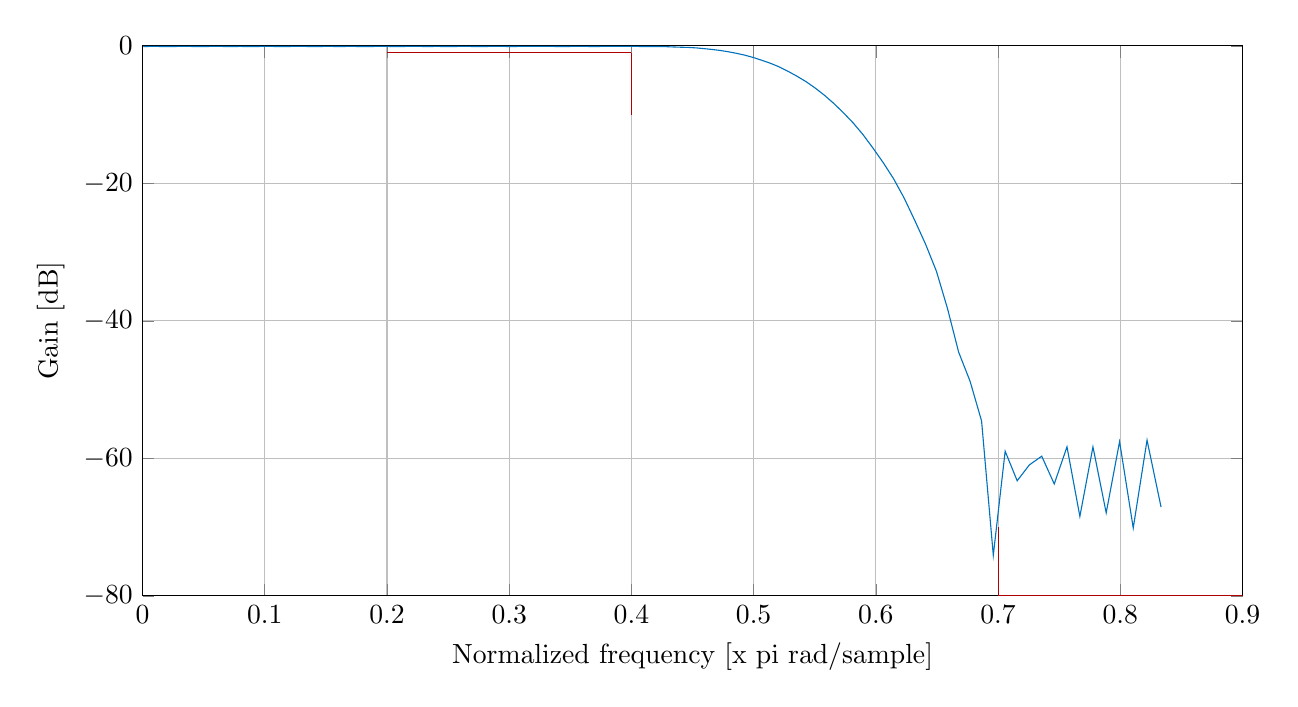
\begin{tikzpicture}

\begin{axis}[%
width=5.5in,
height=2.75in,
at={(0.758in,0.481in)},
scale only axis,
xmin=0,
xmax=0.9,
xlabel={Normalized frequency [x pi rad/sample]},
xmajorgrids,
ymin=-80,
ymax=0,
ylabel={Gain [dB]},
ymajorgrids,
axis background/.style={fill=white}
]
\addplot [color=mycolor1,solid,forget plot]
  table[row sep=crcr]{%
0.000833333333333333	-0.097951\\
0.000844958333333333	-0.097948\\
0.000856708333333333	-0.098065\\
0.000868666666666667	-0.097507\\
0.000880791666666667	-0.097993\\
0.000893041666666667	-0.097965\\
0.0009055	-0.097864\\
0.000918125	-0.097139\\
0.000930916666666667	-0.097446\\
0.000943916666666667	-0.097587\\
0.000957041666666667	-0.097317\\
0.000970416666666667	-0.09724\\
0.000983916666666667	-0.09723\\
0.000997625	-0.097373\\
0.00101154166666667	-0.097006\\
0.00102566666666667	-0.097097\\
0.00103995833333333	-0.097171\\
0.00105445833333333	-0.097188\\
0.001069125	-0.096951\\
0.00108404166666667	-0.097089\\
0.00109916666666667	-0.09684\\
0.00111445833333333	-0.096783\\
0.00113	-0.096567\\
0.00114575	-0.096899\\
0.00116175	-0.096688\\
0.00117791666666667	-0.09661\\
0.00119433333333333	-0.096585\\
0.001211	-0.096347\\
0.001227875	-0.096748\\
0.001245	-0.096439\\
0.00126233333333333	-0.09641\\
0.00127995833333333	-0.09646\\
0.00129779166666667	-0.096354\\
0.001315875	-0.096474\\
0.00133420833333333	-0.096499\\
0.00135283333333333	-0.096415\\
0.00137166666666667	-0.096235\\
0.00139079166666667	-0.096396\\
0.00141016666666667	-0.096061\\
0.00142983333333333	-0.096071\\
0.00144979166666667	-0.096415\\
0.00147	-0.09637\\
0.00149045833333333	-0.096074\\
0.00151125	-0.096036\\
0.00153233333333333	-0.095967\\
0.00155366666666667	-0.095946\\
0.00157533333333333	-0.096017\\
0.00159729166666667	-0.096338\\
0.00161954166666667	-0.096056\\
0.001642125	-0.095982\\
0.00166504166666667	-0.096069\\
0.00168825	-0.09552\\
0.00171175	-0.095835\\
0.001735625	-0.095791\\
0.00175983333333333	-0.095799\\
0.00178433333333333	-0.095872\\
0.00180920833333333	-0.095901\\
0.00183445833333333	-0.096089\\
0.00186	-0.09572\\
0.00188595833333333	-0.09591\\
0.00191225	-0.095659\\
0.001938875	-0.095833\\
0.00196591666666667	-0.095778\\
0.00199333333333333	-0.095647\\
0.00202108333333333	-0.095551\\
0.00204929166666667	-0.095494\\
0.00207783333333333	-0.095715\\
0.00210679166666667	-0.095343\\
0.00213616666666667	-0.095551\\
0.00216595833333333	-0.095734\\
0.002196125	-0.095345\\
0.00222675	-0.095303\\
0.00225779166666667	-0.095187\\
0.00228925	-0.095182\\
0.00232116666666667	-0.095441\\
0.00235354166666667	-0.095153\\
0.00238633333333333	-0.095141\\
0.002419625	-0.095265\\
0.00245333333333333	-0.095107\\
0.00248754166666667	-0.095281\\
0.00252220833333333	-0.094865\\
0.002557375	-0.095374\\
0.002593	-0.09514\\
0.00262916666666667	-0.094937\\
0.00266579166666667	-0.094708\\
0.00270295833333333	-0.095265\\
0.002740625	-0.094855\\
0.00277883333333333	-0.094855\\
0.00281758333333333	-0.094647\\
0.002856875	-0.094766\\
0.00289666666666667	-0.094695\\
0.00293704166666667	-0.09527\\
0.002978	-0.094624\\
0.0030195	-0.094796\\
0.00306158333333333	-0.09472\\
0.00310429166666667	-0.094653\\
0.00314754166666667	-0.094619\\
0.00319141666666667	-0.094367\\
0.00323591666666667	-0.094242\\
0.00328104166666667	-0.094603\\
0.00332675	-0.094592\\
0.003373125	-0.093989\\
0.00342016666666667	-0.094412\\
0.00346783333333333	-0.093993\\
0.00351616666666667	-0.094076\\
0.00356516666666667	-0.094319\\
0.003614875	-0.093586\\
0.00366525	-0.093551\\
0.003716375	-0.09395\\
0.00376816666666667	-0.093488\\
0.00382066666666667	-0.093927\\
0.00387395833333333	-0.093942\\
0.00392795833333333	-0.09368\\
0.00398270833333333	-0.093387\\
0.00403820833333333	-0.093492\\
0.0040945	-0.093449\\
0.00415158333333333	-0.093489\\
0.00420958333333333	-0.093389\\
0.00426833333333333	-0.093601\\
0.0043275	-0.092993\\
0.00438791666666667	-0.093715\\
0.00444916666666667	-0.093388\\
0.00451125	-0.092694\\
0.00457416666666667	-0.092859\\
0.00463791666666667	-0.092695\\
0.0047025	-0.092444\\
0.00476791666666667	-0.092893\\
0.00483458333333333	-0.092351\\
0.00490166666666667	-0.092186\\
0.00497	-0.092605\\
0.00503958333333333	-0.091951\\
0.00510958333333333	-0.092032\\
0.00518083333333333	-0.092045\\
0.00525333333333333	-0.091295\\
0.00532625	-0.09189\\
0.00540041666666667	-0.092102\\
0.00547583333333333	-0.091917\\
0.00555208333333333	-0.09185\\
0.00562958333333333	-0.091589\\
0.00570791666666667	-0.092069\\
0.0057875	-0.091265\\
0.00586833333333333	-0.091803\\
0.00595	-0.091643\\
0.00603291666666667	-0.091381\\
0.00611708333333333	-0.091427\\
0.0062025	-0.091269\\
0.00628875	-0.090504\\
0.00637666666666667	-0.091372\\
0.00646541666666667	-0.090922\\
0.00655541666666667	-0.08975\\
0.00664708333333333	-0.091156\\
0.00673958333333333	-0.091001\\
0.00683375	-0.090184\\
0.00692875	-0.090153\\
0.00702541666666667	-0.090896\\
0.00712333333333333	-0.090426\\
0.0072225	-0.089923\\
0.00732333333333333	-0.089193\\
0.00742541666666667	-0.090176\\
0.00752875	-0.09009\\
0.00763375	-0.089353\\
0.00774041666666667	-0.089903\\
0.00784833333333333	-0.089419\\
0.0079575	-0.08948\\
0.00806833333333333	-0.089849\\
0.00818083333333333	-0.08976\\
0.008295	-0.089816\\
0.00841041666666667	-0.089958\\
0.00852791666666667	-0.088681\\
0.00864666666666667	-0.089346\\
0.00876708333333333	-0.089088\\
0.00888958333333333	-0.089281\\
0.00901333333333333	-0.088858\\
0.00913916666666667	-0.088939\\
0.00926625	-0.089423\\
0.00939541666666667	-0.089071\\
0.00952666666666667	-0.088596\\
0.00965916666666667	-0.089114\\
0.00979416666666667	-0.088773\\
0.00993041666666667	-0.089127\\
0.01006875	-0.089492\\
0.0102091666666667	-0.089024\\
0.0103516666666667	-0.08946\\
0.0104958333333333	-0.089356\\
0.0106420833333333	-0.089494\\
0.0107904166666667	-0.089576\\
0.0109408333333333	-0.089583\\
0.0110933333333333	-0.089773\\
0.0112479166666667	-0.090042\\
0.011405	-0.090246\\
0.01156375	-0.089804\\
0.011725	-0.090332\\
0.0118883333333333	-0.090274\\
0.0120541666666667	-0.090594\\
0.0122220833333333	-0.090886\\
0.0123925	-0.091292\\
0.0125654166666667	-0.090951\\
0.0127404166666667	-0.090949\\
0.0129183333333333	-0.092053\\
0.0130983333333333	-0.092038\\
0.0132808333333333	-0.092554\\
0.0134658333333333	-0.092191\\
0.01365375	-0.093356\\
0.01384375	-0.093842\\
0.0140370833333333	-0.093254\\
0.0142325	-0.093607\\
0.0144308333333333	-0.094182\\
0.0146320833333333	-0.094332\\
0.01483625	-0.094633\\
0.0150429166666667	-0.095663\\
0.0152525	-0.095981\\
0.0154654166666667	-0.096493\\
0.0156808333333333	-0.096889\\
0.0158991666666667	-0.096951\\
0.0161208333333333	-0.09828\\
0.0163458333333333	-0.098183\\
0.01657375	-0.099296\\
0.0168045833333333	-0.099054\\
0.01703875	-0.099121\\
0.01727625	-0.10017\\
0.0175170833333333	-0.10039\\
0.01776125	-0.10116\\
0.01800875	-0.10092\\
0.01826	-0.10128\\
0.0185145833333333	-0.10264\\
0.0187725	-0.10199\\
0.0190341666666667	-0.10281\\
0.0192995833333333	-0.10328\\
0.01956875	-0.10387\\
0.01984125	-0.10377\\
0.0201179166666667	-0.10375\\
0.0203983333333333	-0.1046\\
0.0206829166666667	-0.10386\\
0.02097125	-0.10428\\
0.0212633333333333	-0.10457\\
0.0215595833333333	-0.10518\\
0.0218604166666667	-0.10422\\
0.022165	-0.10374\\
0.0224741666666667	-0.10376\\
0.0227870833333333	-0.10348\\
0.023105	-0.10306\\
0.0234270833333333	-0.10266\\
0.02375375	-0.10225\\
0.0240845833333333	-0.10178\\
0.0244204166666667	-0.10131\\
0.0247608333333333	-0.10089\\
0.0251058333333333	-0.1004\\
0.0254558333333333	-0.099454\\
0.0258108333333333	-0.097796\\
0.0261704166666667	-0.096614\\
0.0265354166666667	-0.095915\\
0.0269054166666667	-0.095577\\
0.0272804166666667	-0.094593\\
0.0276604166666667	-0.093519\\
0.02804625	-0.092372\\
0.0284370833333333	-0.091477\\
0.0288333333333333	-0.090293\\
0.0292354166666667	-0.088929\\
0.0296429166666667	-0.08738\\
0.03005625	-0.087087\\
0.030475	-0.08589\\
0.0309	-0.084928\\
0.0313304166666667	-0.083997\\
0.0317675	-0.083214\\
0.03221	-0.081575\\
0.0326591666666667	-0.081429\\
0.0331145833333333	-0.081175\\
0.0335758333333333	-0.081537\\
0.0340441666666667	-0.080315\\
0.03451875	-0.081241\\
0.0349995833333333	-0.081709\\
0.0354875	-0.08199\\
0.0359825	-0.08222\\
0.03648375	-0.083973\\
0.0369925	-0.084455\\
0.0375083333333333	-0.085638\\
0.0380308333333333	-0.087943\\
0.03856125	-0.088246\\
0.03909875	-0.089917\\
0.03964375	-0.092206\\
0.04019625	-0.09336\\
0.0407566666666667	-0.095952\\
0.0413245833333333	-0.097987\\
0.0419	-0.098777\\
0.0424833333333333	-0.10116\\
0.043075	-0.10266\\
0.0436791666666667	-0.10395\\
0.0442875	-0.1052\\
0.0449041666666667	-0.10615\\
0.0455291666666667	-0.10694\\
0.0461625	-0.10748\\
0.0468083333333333	-0.10713\\
0.0474583333333333	-0.10725\\
0.0481208333333333	-0.10644\\
0.0487916666666667	-0.10617\\
0.0494708333333333	-0.10416\\
0.0501625	-0.10307\\
0.0508625	-0.10217\\
0.0515708333333333	-0.099737\\
0.0522875	-0.097972\\
0.0530166666666667	-0.095593\\
0.0537583333333333	-0.094096\\
0.0545083333333333	-0.091952\\
0.0552666666666667	-0.089503\\
0.0560375	-0.087925\\
0.0568166666666667	-0.085958\\
0.0576083333333333	-0.085082\\
0.0584125	-0.085253\\
0.0592291666666667	-0.08413\\
0.0600541666666667	-0.08447\\
0.0608916666666667	-0.085474\\
0.0617375	-0.085772\\
0.0626	-0.087167\\
0.0634708333333333	-0.088198\\
0.0643583333333333	-0.089803\\
0.0652541666666667	-0.091626\\
0.0661625	-0.093351\\
0.0670875	-0.095439\\
0.0680208333333333	-0.096399\\
0.0689708333333333	-0.097571\\
0.0699291666666667	-0.097936\\
0.0709041666666667	-0.098725\\
0.0718916666666667	-0.098437\\
0.0728958333333333	-0.098251\\
0.0739125	-0.096978\\
0.0749416666666667	-0.095984\\
0.0759875	-0.095233\\
0.0770458333333333	-0.094288\\
0.0781208333333333	-0.092744\\
0.0792083333333333	-0.092461\\
0.0803125	-0.091917\\
0.0814333333333333	-0.092547\\
0.0825666666666667	-0.093461\\
0.0837208333333333	-0.093797\\
0.0848875	-0.09506\\
0.0860708333333333	-0.096272\\
0.0872708333333333	-0.097922\\
0.0884833333333333	-0.098876\\
0.0897166666666667	-0.099333\\
0.0909708333333333	-0.099722\\
0.0922375	-0.098069\\
0.093525	-0.096675\\
0.094825	-0.094033\\
0.09615	-0.092042\\
0.0974875	-0.089115\\
0.0988458333333333	-0.086554\\
0.100225	-0.084779\\
0.101620833333333	-0.083713\\
0.1030375	-0.084658\\
0.104475	-0.085634\\
0.105933333333333	-0.088585\\
0.107408333333333	-0.093114\\
0.108904166666667	-0.096102\\
0.110425	-0.10134\\
0.1119625	-0.10439\\
0.113525	-0.10681\\
0.115108333333333	-0.10681\\
0.1167125	-0.10541\\
0.1183375	-0.10145\\
0.1199875	-0.097021\\
0.121658333333333	-0.0915\\
0.123354166666667	-0.086303\\
0.125075	-0.08226\\
0.126820833333333	-0.081112\\
0.1285875	-0.081356\\
0.130379166666667	-0.083311\\
0.132195833333333	-0.087256\\
0.1340375	-0.092077\\
0.135908333333333	-0.097867\\
0.1378	-0.10027\\
0.139725	-0.10309\\
0.141670833333333	-0.10189\\
0.143645833333333	-0.098877\\
0.145645833333333	-0.095282\\
0.147679166666667	-0.092598\\
0.1497375	-0.090253\\
0.151825	-0.08988\\
0.153941666666667	-0.090454\\
0.1560875	-0.092759\\
0.1582625	-0.094879\\
0.160466666666667	-0.095816\\
0.162704166666667	-0.095503\\
0.164970833333333	-0.094203\\
0.167270833333333	-0.091392\\
0.169604166666667	-0.090011\\
0.171966666666667	-0.089641\\
0.174366666666667	-0.092287\\
0.176795833333333	-0.098243\\
0.179258333333333	-0.10252\\
0.181758333333333	-0.10573\\
0.184291666666667	-0.10542\\
0.1868625	-0.10077\\
0.189466666666667	-0.091964\\
0.192108333333333	-0.085286\\
0.194783333333333	-0.080447\\
0.1975	-0.082039\\
0.200254166666667	-0.087792\\
0.203045833333333	-0.096949\\
0.205875	-0.10299\\
0.208745833333333	-0.10493\\
0.211654166666667	-0.1003\\
0.214604166666667	-0.092598\\
0.217595833333333	-0.085397\\
0.220629166666667	-0.081637\\
0.223704166666667	-0.084266\\
0.226825	-0.090412\\
0.2299875	-0.094206\\
0.233191666666667	-0.095582\\
0.236441666666667	-0.093942\\
0.2397375	-0.091099\\
0.243079166666667	-0.092334\\
0.246466666666667	-0.095937\\
0.249904166666667	-0.098912\\
0.2533875	-0.099518\\
0.256920833333333	-0.093646\\
0.2605	-0.086484\\
0.264133333333333	-0.083796\\
0.2678125	-0.089623\\
0.271545833333333	-0.10017\\
0.275333333333333	-0.10752\\
0.279170833333333	-0.10277\\
0.2830625	-0.090771\\
0.287008333333333	-0.079517\\
0.291008333333333	-0.079204\\
0.2950625	-0.088393\\
0.299179166666667	-0.097099\\
0.303345833333333	-0.097938\\
0.307575	-0.090895\\
0.3118625	-0.086543\\
0.3162125	-0.08857\\
0.320620833333333	-0.09195\\
0.3250875	-0.091616\\
0.329620833333333	-0.086\\
0.3342125	-0.08704\\
0.338875	-0.096555\\
0.343595833333333	-0.10394\\
0.3483875	-0.096998\\
0.353241666666667	-0.08231\\
0.358166666666667	-0.07711\\
0.363158333333333	-0.088619\\
0.368220833333333	-0.10069\\
0.373354166666667	-0.095405\\
0.378558333333333	-0.081479\\
0.3838375	-0.078146\\
0.3891875	-0.086138\\
0.3946125	-0.090671\\
0.4001125	-0.086851\\
0.4056875	-0.091477\\
0.411345833333333	-0.10337\\
0.417083333333333	-0.10723\\
0.422875	-0.10624\\
0.428791666666667	-0.12755\\
0.43475	-0.17143\\
0.440833333333333	-0.20798\\
0.446958333333333	-0.23907\\
0.453208333333333	-0.30588\\
0.4595	-0.4125\\
0.465916666666667	-0.53093\\
0.472416666666667	-0.67011\\
0.479	-0.85708\\
0.485666666666667	-1.0818\\
0.492458333333333	-1.347\\
0.499333333333333	-1.6835\\
0.506291666666667	-2.0797\\
0.513333333333333	-2.5129\\
0.5205	-3.0331\\
0.52775	-3.673\\
0.535083333333333	-4.3832\\
0.542541666666667	-5.1773\\
0.550125	-6.1103\\
0.557791666666667	-7.1732\\
0.565583333333333	-8.3837\\
0.573458333333333	-9.7383\\
0.581458333333333	-11.224\\
0.589541666666667	-12.934\\
0.59775	-14.904\\
0.606083333333333	-17.013\\
0.614541666666667	-19.349\\
0.623125	-22.142\\
0.631791666666667	-25.384\\
0.640625	-28.836\\
0.649541666666667	-32.783\\
0.658583333333333	-38.196\\
0.66775	-44.569\\
0.677083333333333	-48.79\\
0.6865	-54.576\\
0.696083333333333	-74.099\\
0.705791666666667	-58.975\\
0.715625	-63.27\\
0.725583333333333	-60.965\\
0.735708333333333	-59.692\\
0.745958333333333	-63.732\\
0.756375	-58.329\\
0.766916666666667	-68.454\\
0.777625	-58.34\\
0.788458333333333	-67.934\\
0.799416666666667	-57.572\\
0.810583333333333	-70.138\\
0.821875	-57.365\\
0.833333333333333	-67.083\\
};
\addplot [color=black!30!red,solid,forget plot]
  table[row sep=crcr]{%
0.4	-10\\
0.4	-1\\
};
\addplot [color=black!30!red,solid,forget plot]
  table[row sep=crcr]{%
0.2	-1\\
0.4	-1\\
};
\addplot [color=black!30!red,solid,forget plot]
  table[row sep=crcr]{%
0.7	-80\\
0.7	-70\\
};
\addplot [color=black!30!red,solid,forget plot]
  table[row sep=crcr]{%
0.7	-80\\
0.9	-80\\
};
\end{axis}
\end{tikzpicture}%
	\caption{Decimation magnitude response with requirements.}
	\label{fig:acceptIntMag}
\end{figure}
\begin{figure}[H]
	\centering
	\tikzsetnextfilename{acceptIntPhase}
	% This file was created by matlab2tikz.
%
%The latest updates can be retrieved from
%  http://www.mathworks.com/matlabcentral/fileexchange/22022-matlab2tikz-matlab2tikz
%where you can also make suggestions and rate matlab2tikz.
%
\definecolor{mycolor1}{rgb}{0.00000,0.44700,0.74100}%
%
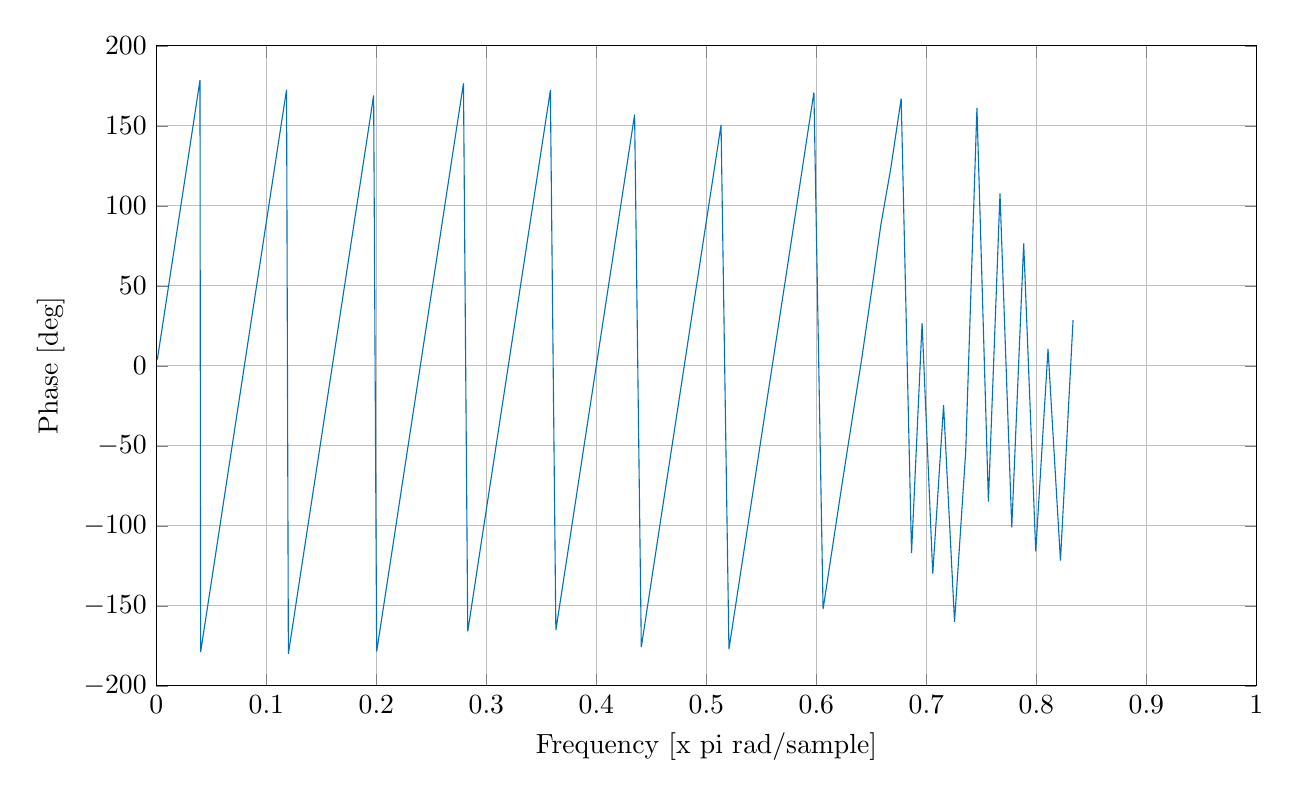
\begin{tikzpicture}

\begin{axis}[%
width=5.5in,
height=3.2in,
at={(0.758in,0.481in)},
scale only axis,
xmin=0,
xmax=1,
xlabel={Frequency [x pi rad/sample]},
xmajorgrids,
ymin=-200,
ymax=200,
ylabel={Phase [deg]},
ymajorgrids,
axis background/.style={fill=white}
]
\addplot [color=mycolor1,solid,forget plot]
  table[row sep=crcr]{%
0.000833333333333333	3.8405\\
0.000844958333333333	3.8925\\
0.000856708333333333	3.9421\\
0.000868666666666667	3.9996\\
0.000880791666666667	4.0513\\
0.000893041666666667	4.1022\\
0.0009055	4.1569\\
0.000918125	4.2158\\
0.000930916666666667	4.2689\\
0.000943916666666667	4.33\\
0.000957041666666667	4.385\\
0.000970416666666667	4.4441\\
0.000983916666666667	4.5025\\
0.000997625	4.5641\\
0.00101154166666667	4.6249\\
0.00102566666666667	4.6878\\
0.00103995833333333	4.7517\\
0.00105445833333333	4.8167\\
0.001069125	4.8804\\
0.00108404166666667	4.9476\\
0.00109916666666667	5.014\\
0.00111445833333333	5.081\\
0.00113	5.1487\\
0.00114575	5.2206\\
0.00116175	5.2906\\
0.00117791666666667	5.363\\
0.00119433333333333	5.4364\\
0.001211	5.5085\\
0.001227875	5.5849\\
0.001245	5.6609\\
0.00126233333333333	5.738\\
0.00127995833333333	5.8139\\
0.00129779166666667	5.8947\\
0.001315875	5.9772\\
0.00133420833333333	6.0558\\
0.00135283333333333	6.1407\\
0.00137166666666667	6.2268\\
0.00139079166666667	6.3105\\
0.00141016666666667	6.3967\\
0.00142983333333333	6.4835\\
0.00144979166666667	6.5719\\
0.00147	6.6611\\
0.00149045833333333	6.7562\\
0.00151125	6.8457\\
0.00153233333333333	6.9395\\
0.00155366666666667	7.0381\\
0.00157533333333333	7.1329\\
0.00159729166666667	7.2296\\
0.00161954166666667	7.3308\\
0.001642125	7.4323\\
0.00166504166666667	7.5325\\
0.00168825	7.6359\\
0.00171175	7.7405\\
0.001735625	7.8499\\
0.00175983333333333	7.9542\\
0.00178433333333333	8.0665\\
0.00180920833333333	8.1737\\
0.00183445833333333	8.291\\
0.00186	8.4048\\
0.00188595833333333	8.521\\
0.00191225	8.6379\\
0.001938875	8.7594\\
0.00196591666666667	8.8775\\
0.00199333333333333	9.0025\\
0.00202108333333333	9.1269\\
0.00204929166666667	9.2507\\
0.00207783333333333	9.3786\\
0.00210679166666667	9.5087\\
0.00213616666666667	9.6399\\
0.00216595833333333	9.7742\\
0.002196125	9.9095\\
0.00222675	10.045\\
0.00225779166666667	10.184\\
0.00228925	10.325\\
0.00232116666666667	10.471\\
0.00235354166666667	10.613\\
0.00238633333333333	10.762\\
0.002419625	10.91\\
0.00245333333333333	11.063\\
0.00248754166666667	11.213\\
0.00252220833333333	11.37\\
0.002557375	11.527\\
0.002593	11.687\\
0.00262916666666667	11.851\\
0.00266579166666667	12.013\\
0.00270295833333333	12.182\\
0.002740625	12.351\\
0.00277883333333333	12.519\\
0.00281758333333333	12.698\\
0.002856875	12.871\\
0.00289666666666667	13.05\\
0.00293704166666667	13.233\\
0.002978	13.416\\
0.0030195	13.602\\
0.00306158333333333	13.79\\
0.00310429166666667	13.983\\
0.00314754166666667	14.177\\
0.00319141666666667	14.374\\
0.00323591666666667	14.571\\
0.00328104166666667	14.776\\
0.00332675	14.98\\
0.003373125	15.191\\
0.00342016666666667	15.4\\
0.00346783333333333	15.614\\
0.00351616666666667	15.832\\
0.00356516666666667	16.051\\
0.003614875	16.276\\
0.00366525	16.504\\
0.003716375	16.733\\
0.00376816666666667	16.962\\
0.00382066666666667	17.199\\
0.00387395833333333	17.437\\
0.00392795833333333	17.683\\
0.00398270833333333	17.925\\
0.00403820833333333	18.178\\
0.0040945	18.433\\
0.00415158333333333	18.688\\
0.00420958333333333	18.947\\
0.00426833333333333	19.21\\
0.0043275	19.48\\
0.00438791666666667	19.751\\
0.00444916666666667	20.025\\
0.00451125	20.307\\
0.00457416666666667	20.589\\
0.00463791666666667	20.875\\
0.0047025	21.167\\
0.00476791666666667	21.462\\
0.00483458333333333	21.757\\
0.00490166666666667	22.064\\
0.00497	22.368\\
0.00503958333333333	22.679\\
0.00510958333333333	22.996\\
0.00518083333333333	23.32\\
0.00525333333333333	23.64\\
0.00532625	23.97\\
0.00540041666666667	24.302\\
0.00547583333333333	24.646\\
0.00555208333333333	24.988\\
0.00562958333333333	25.336\\
0.00570791666666667	25.687\\
0.0057875	26.05\\
0.00586833333333333	26.407\\
0.00595	26.78\\
0.00603291666666667	27.152\\
0.00611708333333333	27.531\\
0.0062025	27.916\\
0.00628875	28.306\\
0.00637666666666667	28.697\\
0.00646541666666667	29.099\\
0.00655541666666667	29.506\\
0.00664708333333333	29.918\\
0.00673958333333333	30.337\\
0.00683375	30.758\\
0.00692875	31.186\\
0.00702541666666667	31.625\\
0.00712333333333333	32.067\\
0.0072225	32.512\\
0.00732333333333333	32.963\\
0.00742541666666667	33.429\\
0.00752875	33.89\\
0.00763375	34.364\\
0.00774041666666667	34.846\\
0.00784833333333333	35.332\\
0.0079575	35.823\\
0.00806833333333333	36.321\\
0.00818083333333333	36.829\\
0.008295	37.347\\
0.00841041666666667	37.867\\
0.00852791666666667	38.398\\
0.00864666666666667	38.932\\
0.00876708333333333	39.474\\
0.00888958333333333	40.025\\
0.00901333333333333	40.587\\
0.00913916666666667	41.152\\
0.00926625	41.726\\
0.00939541666666667	42.309\\
0.00952666666666667	42.899\\
0.00965916666666667	43.499\\
0.00979416666666667	44.107\\
0.00993041666666667	44.726\\
0.01006875	45.343\\
0.0102091666666667	45.981\\
0.0103516666666667	46.619\\
0.0104958333333333	47.269\\
0.0106420833333333	47.934\\
0.0107904166666667	48.596\\
0.0109408333333333	49.277\\
0.0110933333333333	49.968\\
0.0112479166666667	50.66\\
0.011405	51.372\\
0.01156375	52.086\\
0.011725	52.815\\
0.0118883333333333	53.549\\
0.0120541666666667	54.297\\
0.0122220833333333	55.06\\
0.0123925	55.825\\
0.0125654166666667	56.604\\
0.0127404166666667	57.39\\
0.0129183333333333	58.188\\
0.0130983333333333	59.005\\
0.0132808333333333	59.824\\
0.0134658333333333	60.663\\
0.01365375	61.504\\
0.01384375	62.364\\
0.0140370833333333	63.239\\
0.0142325	64.115\\
0.0144308333333333	65.008\\
0.0146320833333333	65.914\\
0.01483625	66.835\\
0.0150429166666667	67.764\\
0.0152525	68.708\\
0.0154654166666667	69.664\\
0.0156808333333333	70.635\\
0.0158991666666667	71.62\\
0.0161208333333333	72.619\\
0.0163458333333333	73.625\\
0.01657375	74.647\\
0.0168045833333333	75.686\\
0.01703875	76.742\\
0.01727625	77.81\\
0.0175170833333333	78.892\\
0.01776125	79.987\\
0.01800875	81.104\\
0.01826	82.231\\
0.0185145833333333	83.375\\
0.0187725	84.525\\
0.0190341666666667	85.707\\
0.0192995833333333	86.896\\
0.01956875	88.101\\
0.01984125	89.325\\
0.0201179166666667	90.569\\
0.0203983333333333	91.827\\
0.0206829166666667	93.101\\
0.02097125	94.397\\
0.0212633333333333	95.707\\
0.0215595833333333	97.032\\
0.0218604166666667	98.382\\
0.022165	99.747\\
0.0224741666666667	101.14\\
0.0227870833333333	102.54\\
0.023105	103.96\\
0.0234270833333333	105.4\\
0.02375375	106.88\\
0.0240845833333333	108.36\\
0.0244204166666667	109.87\\
0.0247608333333333	111.39\\
0.0251058333333333	112.94\\
0.0254558333333333	114.51\\
0.0258108333333333	116.11\\
0.0261704166666667	117.73\\
0.0265354166666667	119.37\\
0.0269054166666667	121.03\\
0.0272804166666667	122.72\\
0.0276604166666667	124.43\\
0.02804625	126.16\\
0.0284370833333333	127.93\\
0.0288333333333333	129.71\\
0.0292354166666667	131.52\\
0.0296429166666667	133.36\\
0.03005625	135.23\\
0.030475	137.11\\
0.0309	139.04\\
0.0313304166666667	140.98\\
0.0317675	142.95\\
0.03221	144.96\\
0.0326591666666667	146.98\\
0.0331145833333333	149.04\\
0.0335758333333333	151.13\\
0.0340441666666667	153.25\\
0.03451875	155.39\\
0.0349995833333333	157.57\\
0.0354875	159.77\\
0.0359825	162.01\\
0.03648375	164.28\\
0.0369925	166.57\\
0.0375083333333333	168.9\\
0.0380308333333333	171.26\\
0.03856125	173.65\\
0.03909875	176.08\\
0.03964375	178.53\\
0.04019625	-178.98\\
0.0407566666666667	-176.45\\
0.0413245833333333	-173.9\\
0.0419	-171.31\\
0.0424833333333333	-168.69\\
0.043075	-166.03\\
0.0436791666666667	-163.34\\
0.0442875	-160.61\\
0.0449041666666667	-157.84\\
0.0455291666666667	-155.03\\
0.0461625	-152.18\\
0.0468083333333333	-149.31\\
0.0474583333333333	-146.38\\
0.0481208333333333	-143.42\\
0.0487916666666667	-140.41\\
0.0494708333333333	-137.36\\
0.0501625	-134.26\\
0.0508625	-131.13\\
0.0515708333333333	-127.95\\
0.0522875	-124.71\\
0.0530166666666667	-121.43\\
0.0537583333333333	-118.1\\
0.0545083333333333	-114.73\\
0.0552666666666667	-111.3\\
0.0560375	-107.83\\
0.0568166666666667	-104.3\\
0.0576083333333333	-100.73\\
0.0584125	-97.096\\
0.0592291666666667	-93.421\\
0.0600541666666667	-89.693\\
0.0608916666666667	-85.914\\
0.0617375	-82.08\\
0.0626	-78.191\\
0.0634708333333333	-74.263\\
0.0643583333333333	-70.274\\
0.0652541666666667	-66.235\\
0.0661625	-62.144\\
0.0670875	-57.988\\
0.0680208333333333	-53.787\\
0.0689708333333333	-49.53\\
0.0699291666666667	-45.21\\
0.0709041666666667	-40.832\\
0.0718916666666667	-36.393\\
0.0728958333333333	-31.89\\
0.0739125	-27.322\\
0.0749416666666667	-22.69\\
0.0759875	-17.988\\
0.0770458333333333	-13.217\\
0.0781208333333333	-8.3809\\
0.0792083333333333	-3.4751\\
0.0803125	1.5041\\
0.0814333333333333	6.5454\\
0.0825666666666667	11.663\\
0.0837208333333333	16.849\\
0.0848875	22.104\\
0.0860708333333333	27.427\\
0.0872708333333333	32.821\\
0.0884833333333333	38.288\\
0.0897166666666667	43.829\\
0.0909708333333333	49.446\\
0.0922375	55.142\\
0.093525	60.923\\
0.094825	66.78\\
0.09615	72.73\\
0.0974875	78.769\\
0.0988458333333333	84.894\\
0.100225	91.117\\
0.101620833333333	97.427\\
0.1030375	103.83\\
0.104475	110.31\\
0.105933333333333	116.89\\
0.107408333333333	123.55\\
0.108904166666667	130.29\\
0.110425	137.11\\
0.1119625	144.02\\
0.113525	151.02\\
0.115108333333333	158.11\\
0.1167125	165.3\\
0.1183375	172.6\\
0.1199875	-179.99\\
0.121658333333333	-172.47\\
0.123354166666667	-164.82\\
0.125075	-157.06\\
0.126820833333333	-149.18\\
0.1285875	-141.18\\
0.130379166666667	-133.09\\
0.132195833333333	-124.89\\
0.1340375	-116.59\\
0.135908333333333	-108.19\\
0.1378	-99.682\\
0.139725	-91.063\\
0.141670833333333	-82.331\\
0.143645833333333	-73.465\\
0.145645833333333	-64.462\\
0.147679166666667	-55.321\\
0.1497375	-46.039\\
0.151825	-36.627\\
0.153941666666667	-27.085\\
0.1560875	-17.416\\
0.1582625	-7.6308\\
0.160466666666667	2.2884\\
0.162704166666667	12.344\\
0.164970833333333	22.545\\
0.167270833333333	32.906\\
0.169604166666667	43.417\\
0.171966666666667	54.082\\
0.174366666666667	64.897\\
0.176795833333333	75.847\\
0.179258333333333	86.924\\
0.181758333333333	98.144\\
0.184291666666667	109.5\\
0.1868625	121.03\\
0.189466666666667	132.75\\
0.192108333333333	144.66\\
0.194783333333333	156.76\\
0.1975	169.04\\
0.200254166666667	-178.53\\
0.203045833333333	-165.96\\
0.205875	-153.26\\
0.208745833333333	-140.4\\
0.211654166666667	-127.35\\
0.214604166666667	-114.09\\
0.217595833333333	-100.61\\
0.220629166666667	-86.915\\
0.223704166666667	-73.034\\
0.226825	-58.981\\
0.2299875	-44.764\\
0.233191666666667	-30.361\\
0.236441666666667	-15.746\\
0.2397375	-0.91004\\
0.243079166666667	14.157\\
0.246466666666667	29.418\\
0.249904166666667	44.861\\
0.2533875	60.508\\
0.256920833333333	76.386\\
0.2605	92.531\\
0.264133333333333	108.93\\
0.2678125	125.57\\
0.271545833333333	142.37\\
0.275333333333333	159.35\\
0.279170833333333	176.55\\
0.2830625	-165.96\\
0.287008333333333	-148.15\\
0.291008333333333	-130.07\\
0.2950625	-111.77\\
0.299179166666667	-93.296\\
0.303345833333333	-74.588\\
0.307575	-55.58\\
0.3118625	-36.266\\
0.3162125	-16.669\\
0.320620833333333	3.1611\\
0.3250875	23.258\\
0.329620833333333	43.662\\
0.3342125	64.404\\
0.338875	85.4\\
0.343595833333333	106.61\\
0.3483875	128.09\\
0.353241666666667	149.96\\
0.358166666666667	172.23\\
0.363158333333333	-165.24\\
0.368220833333333	-142.51\\
0.373354166666667	-119.51\\
0.378558333333333	-96.088\\
0.3838375	-72.268\\
0.3891875	-48.163\\
0.3946125	-23.785\\
0.4001125	0.96562\\
0.4056875	26.112\\
0.411345833333333	51.543\\
0.417083333333333	77.295\\
0.422875	103.5\\
0.428791666666667	130.15\\
0.43475	157.03\\
0.440833333333333	-175.81\\
0.446958333333333	-148.15\\
0.453208333333333	-120\\
0.4595	-91.558\\
0.465916666666667	-62.815\\
0.472416666666667	-33.588\\
0.479	-3.9171\\
0.485666666666667	26.105\\
0.492458333333333	56.619\\
0.499333333333333	87.597\\
0.506291666666667	118.84\\
0.513333333333333	150.54\\
0.5205	-177.1\\
0.52775	-144.41\\
0.535083333333333	-111.46\\
0.542541666666667	-77.904\\
0.550125	-43.798\\
0.557791666666667	-9.2722\\
0.565583333333333	25.719\\
0.573458333333333	61.108\\
0.581458333333333	97.111\\
0.589541666666667	133.97\\
0.59775	170.88\\
0.606083333333333	-152.05\\
0.614541666666667	-113.75\\
0.623125	-74.831\\
0.631791666666667	-36.578\\
0.640625	1.7888\\
0.649541666666667	43.687\\
0.658583333333333	87.992\\
0.66775	123.93\\
0.677083333333333	167.02\\
0.6865	-117.12\\
0.696083333333333	26.707\\
0.705791666666667	-129.88\\
0.715625	-24.578\\
0.725583333333333	-159.95\\
0.735708333333333	-54.032\\
0.745958333333333	161.14\\
0.756375	-84.874\\
0.766916666666667	107.69\\
0.777625	-100.97\\
0.788458333333333	76.557\\
0.799416666666667	-115.93\\
0.810583333333333	10.53\\
0.821875	-121.78\\
0.833333333333333	28.502\\
};
\end{axis}
\end{tikzpicture}%
	\caption{Decimation Phase response .}
	\label{fig:AcceptIntPhase}
\end{figure}


\subsection*{Compare test}


\section{Error sources}
The generator on the NI-4461 card has a deviation of $\pm$ 0,008 dB from 20 Hz - 20 kHz. The analyzer on the NI-4461 card has a deviation of : $\pm$ 0,08 dB from 20 Hz - 92 kHz. 

\section{Conclusion}
It can be concluded from the two test that both filters meet their respective requirements. They both attenuate enough and have a linear phase with a constant group delay.